\chapter{Agreement Between Experimental and Simulated Circular Dichroic Spectra of a Positively Charged Peptide in Aqueous Solution and on Self-Assembled Monolayers}\label{helix-folding}

\newcommand{\tbawat}{{2:1 \emph{t}-BuOH/\ce{H2O}}}
\newcommand{\tba}{{\emph{t}-BuOH}}
\newcommand{\pep}{{\textalpha{}11LK(CH)}}

%Successfully immobilizing functional proteins on inorganic surfaces has long been a challenge to the biophysics and bioengineering communities. 
%This is due in part to a lack of understanding of the effect of non-aqueous environments on protein structure from both experimental and computational perspectives. 
%Because most experimental information about protein structure comes from the protein data bank (PDB) and is collected from an aqueous solvent environment, modern force fields for molecular dynamics (MD) simulations are parameterized against these data. 
%Therefore, the applicability of such force fields to biomolecules in different environments, including when in contact with surfaces and substrates, must be validated. 
%Here, we present MD folding simulations of a highly charged peptide solvated in water, solvated in a solution of \tbawat{}, and bound to the surface of a methyl-terminated self-assembled monolayer (SAM) and compare the structures predicted by these simulations to previously reported circular dichroism (CD) spectra. 
%We show quantitative agreement between experiment and simulation of solvent- and surface-induced conformational changes of a positively charged peptide in these three environments. 
%We show further that that the surface-bound peptide must fold before chemically reacting with the surface. 
%Finally, we demonstrate that a well-ordered SAM is critical to the folding process. 
%These results will guide further simulations of peptides and proteins in diverse and complex environments. 

%%%%%%%%%%%%%%%%%%%%%%%%%%%%%%%%%%%%%%%%%%%%%%%%%%%%%%%%%%%%%%%%
%%%%%%%%%%%%%%%%%%%%%%%%%%%%%%%%%%%%%%%%%%%%%%%%%%%%%%%%%%%%%%%%
\section{Publication note} \label{helix-pub-note}
%%%%%%%%%%%%%%%%%%%%%%%%%%%%%%%%%%%%%%%%%%%%%%%%%%%%%%%%%%%%%%%%
%%%%%%%%%%%%%%%%%%%%%%%%%%%%%%%%%%%%%%%%%%%%%%%%%%%%%%%%%%%%%%%%

Portions of this chapter are adapted from the following publication: 

\noindent Jeremy T. First, Lauren J. Webb; Agreement Between Experimental and Simulated Circular Dichroic Spectra of a Positively Charged Peptide in Aqueous Solution and on Self-Assembled Monolayers. \emph{Journal of Physical Chemistry B}. \textbf{2019}, \emph{123}, 4512-4526.

JTF performed all calculations and analyses. 
All code, force field parameters, structures, and other starting files used for the simulation, analysis, processing of data, and figure generation can be accessed at:
\url{https://github.com/jeremyfirst22/GMX_Helix_oplsaa}. 

%%%%%%%%%%%%%%%%%%%%%%%%%%%%%%%%%%%%%%%%%%%%%%%%%%%%%%%%%%%%%%%%
%%%%%%%%%%%%%%%%%%%%%%%%%%%%%%%%%%%%%%%%%%%%%%%%%%%%%%%%%%%%%%%%
\section{Introduction}\index{helix-intro}
%%%%%%%%%%%%%%%%%%%%%%%%%%%%%%%%%%%%%%%%%%%%%%%%%%%%%%%%%%%%%%%%
%%%%%%%%%%%%%%%%%%%%%%%%%%%%%%%%%%%%%%%%%%%%%%%%%%%%%%%%%%%%%%%%

Quantitatively reliable computer simulations of biomolecular properties such as structure, ligand binding, dynamics, and function are now a ubiquitous aspect of biomolecular research. 
Much of this success is aided by recent dramatic increases in computational resources, computational efficiency, and accuracy of computational methodologies. 
While these methodologies vary in scale and level of physical description, every method must be validated against experimental data. 
Molecular dynamics (MD) simulations rely on a potential energy function (referred to as a force field) that can accurately reproduce structural data in a protein database (PDB). 
In some cases, this has been extremely successful \cite{Duan1998, Lindorff-Larsen2011, Bowman2011, Voelz2012, Shaw2010, Lane2013, Koukos2014a}.
To date, however, over 90\% of structures deposited in the PDB come from X-ray crystallography experiments \cite{Berman2000}. 
This inherently biases the database to systems for which a crystal can be obtained: often compact, globular proteins crystallized from dilute solutions. 
While such structures dominate the PDB, most interesting biological phenomena occur in systems too complex to crystalize. 
For example, structural information of docked protein complexes, protein-surface interactions, protein-membrane interactions, intrinsically disordered proteins, or proteins in non-aqueous environments are currently rare in the PDB\cite{Berman2013} despite the importance of such systems in the living cell. 
The applicability of force field parameters validated against PDB structures to these more complex biological systems is therefore not guaranteed.

The necessity for reliable simulations at or near a surface has recently become more apparent for several reasons. 
First, there is growing evidence of a link between surface-induced conformational changes and the development of diseases associated with amyloid plaques \cite{Makin2005, Rambaran2008, Lednev2014}.
Second, the crowded conditions inside a cell likely preclude proteins from being alone in dilute solvent. 
It has been suggested surfaces, such as the inside of the chaperonin cavity, alter the free energy landscape of folding preventing misfolded intermediates\cite{Bhattacharya2012}, and full atomistic simulations of such large systems have only recently become accessible\cite{Piana2018}. 
Third, from an applications perspective, the growing interest in immobilizing proteins on abiological surfaces for use in biosensors and catalytic devices likewise will require accurate simulations of biomolecular structure and dynamics within these artificial environments to develop and test hypotheses of protein-surface interactions \cite{Sarikaya2003, Barton2004, Noll2011, Renner2016}.
Evolved biological molecules offer specificity and reactivity that has yet to be replicated in artificial devices and could therefore be of enormous benefit to the biomedical community if they could be reliably incorporated onto a device. 
The glucose monitor, which converts blood glucose concentration to an electrochemical readout using glucose oxidase bound to a biochemical sensor, is a well-known example of such a device\cite{Wang2008}. 
However, harnessing biomolecular specificity and reactivity on a device is impeded by the difficulty of immobilizing a protein on an inorganic substrate in a controlled manner while simultaneously maintaining the structure and function of the protein that is heavily dependent on its solvation environment. 
This is further hindered by the lack of general and reliable MD methods to inform surface design and interpret experimental results. 

Experimental work in our laboratory has focused on implementing a two-fold strategy to immobilize proteins on a gold surface in a reproducible and controlled manner: 
1) the use of an organic blocking layer between the protein and the Au surface; and 
2) the covalent attachment of a peptide to the blocking layer, creating a biomimetic surface to immobilize the protein by exploiting native noncovalent and electrostatic interactions. 
To this end, we have covalently attached an alkyne-containing peptide using a Cu(I) catalyzed Huisgen cycloaddition (i.e. ``click'' reaction) with homogenously dispersed \ce{N3}-terminated alkane thiols in a self-assembled monolayer (SAM) of decanethiols\cite{Gallardo2010}.   
Recently, we have demonstrated that similar strategies can be used to attach this peptide on nanoparticles as well\cite{Wilder2019}. 
These surfaces have been characterized extensively through both surface-averaged and spatially-resolved methods\cite{Gallardo2010, Gallardo2012, Raigoza2012, Dugger2015a, Dugger2015, Raigoza2017}.
Reliable MD simulations could aid and inform our experimental design; however, the application of generally available methods to biomolecules in abiological systems, such as non-aqueous solvents or near a surface, requires careful consideration and validation of the computational methodology. 
For example, the Latour group developed a specialized dual force field model to generate simulations that accurately reproduced adsorption energies of peptides on an abiological surface \cite{Latour2002, Raut2005, Abramyan2015}.
However, such methods are not widely available and can require extensive expertise to implement. 
Extending more canonical force fields such as Amber, OPLS, and CHARMM to such environments requires validation against experimental data such as we have collected for the specific peptide-terminated Au surfaces generated in our laboratory.

%Non breaking spaces, '~' added to prevent peptide sequence from overflowing into the margins 
We~ have~ previously~ investigated~ a~ surface-bound~ peptide~ with~ the~ sequence LKKLXKKLLKKLLKKXLKKL, where X is the unnatural amino acid propargylglycine. 
(Hereafter, we refer to the peptide as ``\pep{}''). 
This was designed by DeGrado and Lear to adopt a helical conformation at a polar/apolar interface \cite{DeGrado1985}.   
The spacing of the hydrophilic and hydrophobic residues is such that, when the peptide is perfectly \textalpha{}-helical, the charged lysine residues are one side of the helical axis and the nonpolar leucine residues are on the opposite side of the helical axis. 
Therefore, when the peptide is at a polar/apolar interface, the peptide assumes a helical conformation to maximize contact between the polar residues and the polar solvent, and between the nonpolar residues and the apolar medium\cite{DeGrado1985}. 
In previously published work using circular dichroism (CD) spectroscopy (Figure \ref{fig:helix-cd_spectra}), we observed three distinct spectra of this peptide in three different solvent environments, each with different hydrophobicity \cite{Gallardo2012}.   
When dissolved in aqueous buffer, the observed CD spectrum of \pep{} indicated an unfolded or disordered conformation (Figure \ref{fig:helix-cd_spectra}, black). 
When dissolved in \tbawat{} (the solvent for the ``click'' reaction), the observed CD spectrum contained two unresolved negative features, around 208 nm and 222 nm (Figure \ref{fig:helix-cd_spectra}, blue). 
Negative ellipticity at these wavelengths is indicative of helical character \cite{Holzwarth1965, Woody1967, Johnson1988, Berova2000circular, Kelly2005}.
Because of the relative intensity of these two troughs, we hypothesized that the peptide was in a $3_{10}$-helix or a partially folded \textalpha{}-helical conformation. 
When chemically bound to a SAM on a gold surface, the observed CD spectrum contained similar negative features at 209 nm and 223 nm (Figure \ref{fig:helix-cd_spectra}, green), but with greater resolution between the two peaks, indicating higher helical content when the peptide was bound to the SAM surface than when solvated in either of the two solvents. 

\begin{figure}  
    \center
    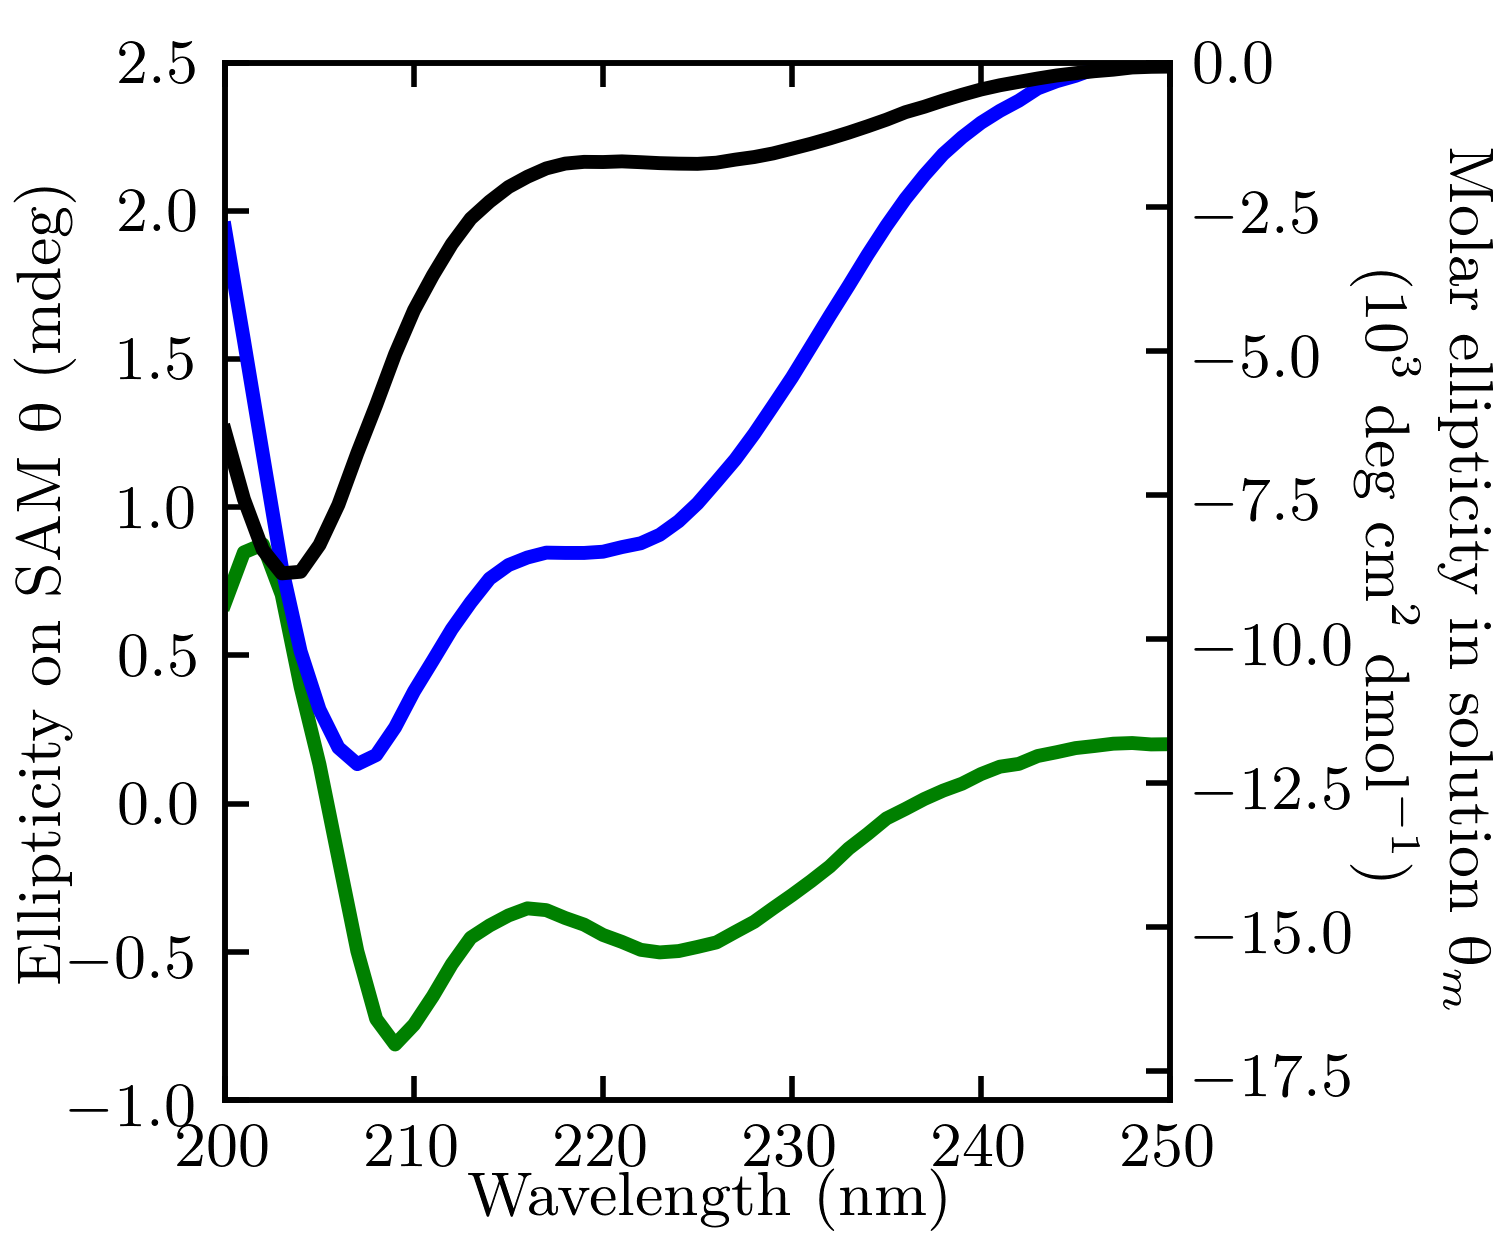
\includegraphics[width=\single]{figures-helix/nachos_cd_spectra.png}
    \caption[Circular dichroism spectra of \pep{} in three different solvent environments]{
        Circular dichroism spectra of \pep{} in three different solvent environments. 
        Black: \pep{} dissolved in aqueous Tris buffer. 
        Blue: \pep{} dissolved in \tbawat{}. 
        Green: \pep{} covalently attached to a SAM of decanethiols on Au. 
        The left vertical axis is the ellipticity for the peptide on the surface, and the right vertical axis is the ellipticity of the peptide in the two solutions. 
        Adapted from ref \citenum{Gallardo2012}.
    }
    \label{fig:helix-cd_spectra}
\end{figure}

Simulating the structural change demonstrated between these two solvents and the surface environment has proven to be a challenge. 
For example, Di Pierro et al. showed that simply by moving from water to the binary solvent, \tbawat{}, the OPLS force field failed to describe the experimental data \cite{DiPierro2015}.   
The authors reoptimized the \tba{} parameters to interact properly with \ce{H2O} by using a refinement algorithm that systematically minimized the difference between experimental Kirkwood-Buff integrals and the radial distribution functions between \tba{} and water \cite{DiPierro2015}. 
Adding the complexity of an inorganic surface to a simulation is an additional challenge \cite{Walsh2017}. 
Although there are several recent successful simulations of a bio/abio interface, these are less common for several reasons \cite{Gianese2009, Meibner2014, Zerze2015, Cannon2015, Krause2017, Prakash2018a, Prakash2018, Sprenger2018}.
Surface simulations require robust experimental data on the structure of the surface in order to construct an atomically accurate model. 
Further, force field parameters of the surface moieties are rare and often not intended to work with biomolecular force fields \cite{Latour2008, Latour2014}.
Polarization effects of metallic surfaces, such as image charges \cite{Heinz2011}, require additional considerations \cite{Iori2009}. 
However, the biomimetic surface strategy implemented in our published work directly addresses many of these challenges. 
Robust structural data of SAMs is available from surface-averaged spectroscopies such as Fourier transform infrared (FTIR), spatially-resolved scanning tunneling microscopy, and theoretical studies; 
parameters for saturated hydrocarbons are readily accessible and can be combined with biomolecular force fields; 
and the SAM mitigates the electrostatic effects of image charges in gold.

Here, we present MD simulations of \pep{} that successfully capture the experimentally measured solvent- and surface-induced conformational change in water, \tbawat{}, and on the surface of a decanethiol SAM. 
Structural assignments were performed with the Define Secondary Structure of Proteins (DSSP) algorithm and show that the simulations quantitatively captured the amount of secondary structure of \pep{} in each of the three environments when compared to deconvolutions of the experimental CD spectra. 
Theoretical CD spectra were calculated from the MD trajectories using DichroCalc and were in qualitative agreement with experiment. 
These simulations demonstrated that the OPLS-AA force field was sufficiently accurate in \tbawat{} and on the surface of a SAM, despite being parameterized for biomolecules in aqueous solution. 
Herein we describe our simulation setup and protocol, followed by an extensive discussion of the results of the simulations and comparison to the experimental spectra\cite{Gallardo2012} reproduced in Figure \ref{fig:helix-cd_spectra}. 
After demonstrating the validity of our simulations, we present an additional set of simulations designed to explore the mechanism of folding of the peptide on the SAM surface and propose two hypotheses that are currently being experimentally tested in our laboratory.

%%%%%%%%%%%%%%%%%%%%%%%%%%%%%%%%%%%%%%%%%%%%%%%%%%%%%%%%%%%%%%%%
%%%%%%%%%%%%%%%%%%%%%%%%%%%%%%%%%%%%%%%%%%%%%%%%%%%%%%%%%%%%%%%%
\section{Methods}\label{helix-methods}
%%%%%%%%%%%%%%%%%%%%%%%%%%%%%%%%%%%%%%%%%%%%%%%%%%%%%%%%%%%%%%%%
%%%%%%%%%%%%%%%%%%%%%%%%%%%%%%%%%%%%%%%%%%%%%%%%%%%%%%%%%%%%%%%%

All code and starting files used for the simulation, analysis, processing of data, and figure generation can be accessed at: 
\url{https://github.com/jeremyfirst22/GMX_Helix_oplsaa}. 

\subsection{System preparation and force field parameters}

A template of \pep{} was created in a \textalpha{}-helical conformation using the Avogadro molecular editing package\cite{Hanwell2012}.
The propargylglycines, which provided the alkyne group for the ``click'' reaction in the experiment, were replaced with glycine residues. 
Because of the short length of the peptide, the N and C termini were neutralized with an acetyl group and amide group, respectively. 
Parameters for the united atom model of \tba{} (Figure \ref{fig:helix-tba}) were adapted for Gromacs from Di Pierro et al \cite{DiPierro2015}.
To validate our implementation of the \tba{} parameters, we calculated the solvent pair correlation functions of a 0.2 mol fraction \tba{} in \ce{H2O} mixture and found that our calculated pair correlation functions matched those reported in Di Pierro et al. (Figure \ref{fig:helix-rdfs}, compare to Figure 6 of ref \citenum{DiPierro2015}). 
Generally, it is best to avoid combining all-atom models with united-atom models; 
however, in this case, the \tba{} parameters were reoptimized explicitly for mixtures with the TIP3P water model. 
While parameters for decanethiols in SAMs have been published and validated before\cite{Godawat2009}, we wanted to use a consistent force field in all three environments. 
Because of this, parameters for decanethiol within the SAM were adapted from existing OPLS-AA parameters for hydrocarbons\cite{Kaminski1994}. 
Using restricted Hartree-Fock calculations in the GAMESS QM software package\cite{Schmidt1993, Gordon2005}, partial charges were attained by minimizing a decanethiol molecule using the 6-31G basis set and fitting charges to the electrostatic potential calculated at the Connolly surface using the 6-31G(d) basis set. 
Derived charges are shown in Figure \ref{fig:helix-charges}. 
All subsequent calculations used the Gromacs 2016.3 molecular dynamics simulation package\cite{Berendsen1995, Lindahl2001, VanDerSpoel2005, Hess2008, Pronk2013, Pall2015, Abraham2015} and the OPLS-AA force field\cite{Jorgensen1996, Kaminski2001} unless otherwise noted.

\begin{figure}
    \center
    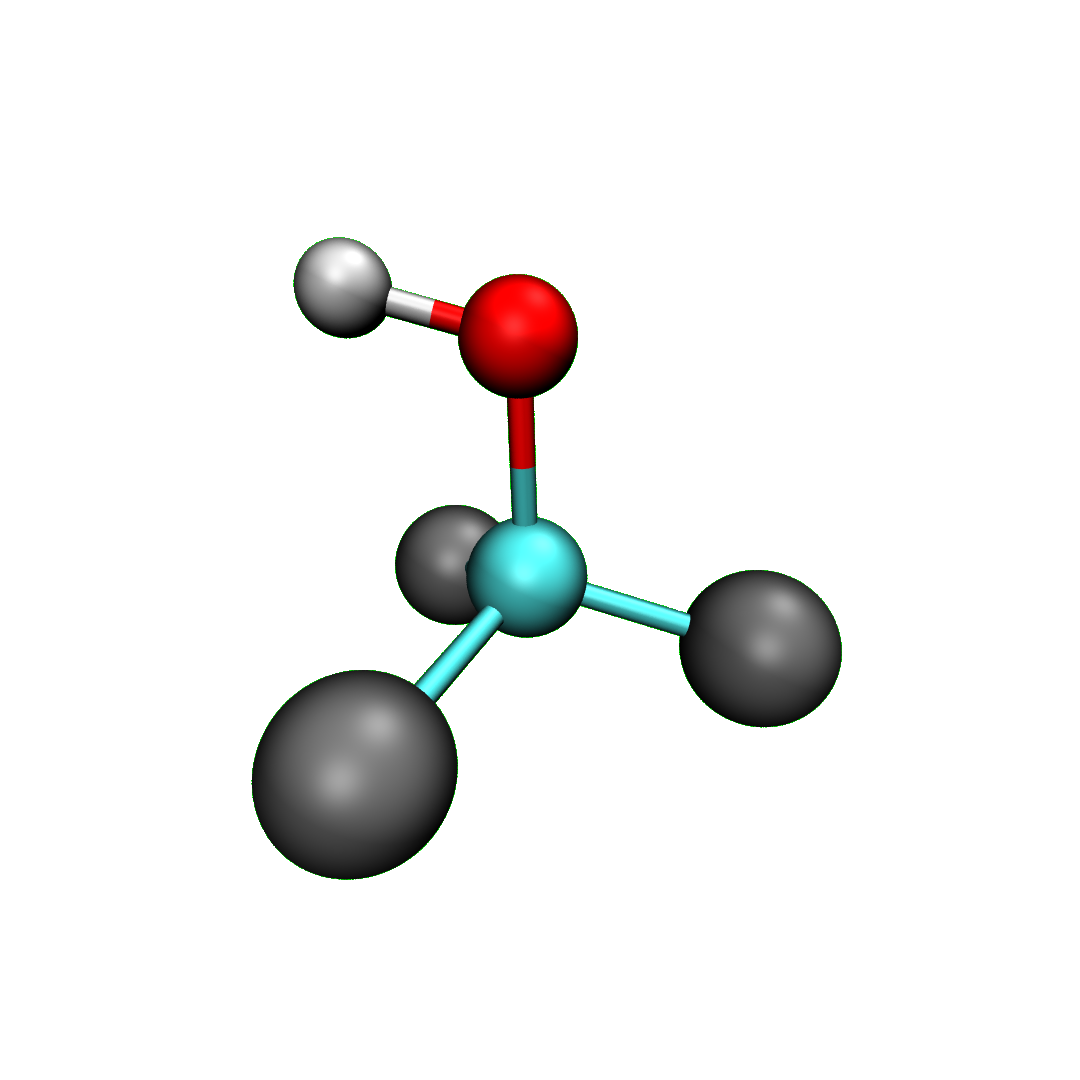
\includegraphics[width=\single]{figures-helix/tba.png}
    \caption[United atom representation of \emph{tert}-butanol]{
        A united atom model of \emph{tert}-butanol used in these simulations. 
        The white sphere represents a hydrogen, the red sphere represents an oxygen, the cyan sphere represents the central carbon, and the gray spheres are united-atom representations of the three methyl groups.
    }
    \label{fig:helix-tba}
\end{figure}

\begin{figure}
    \center
    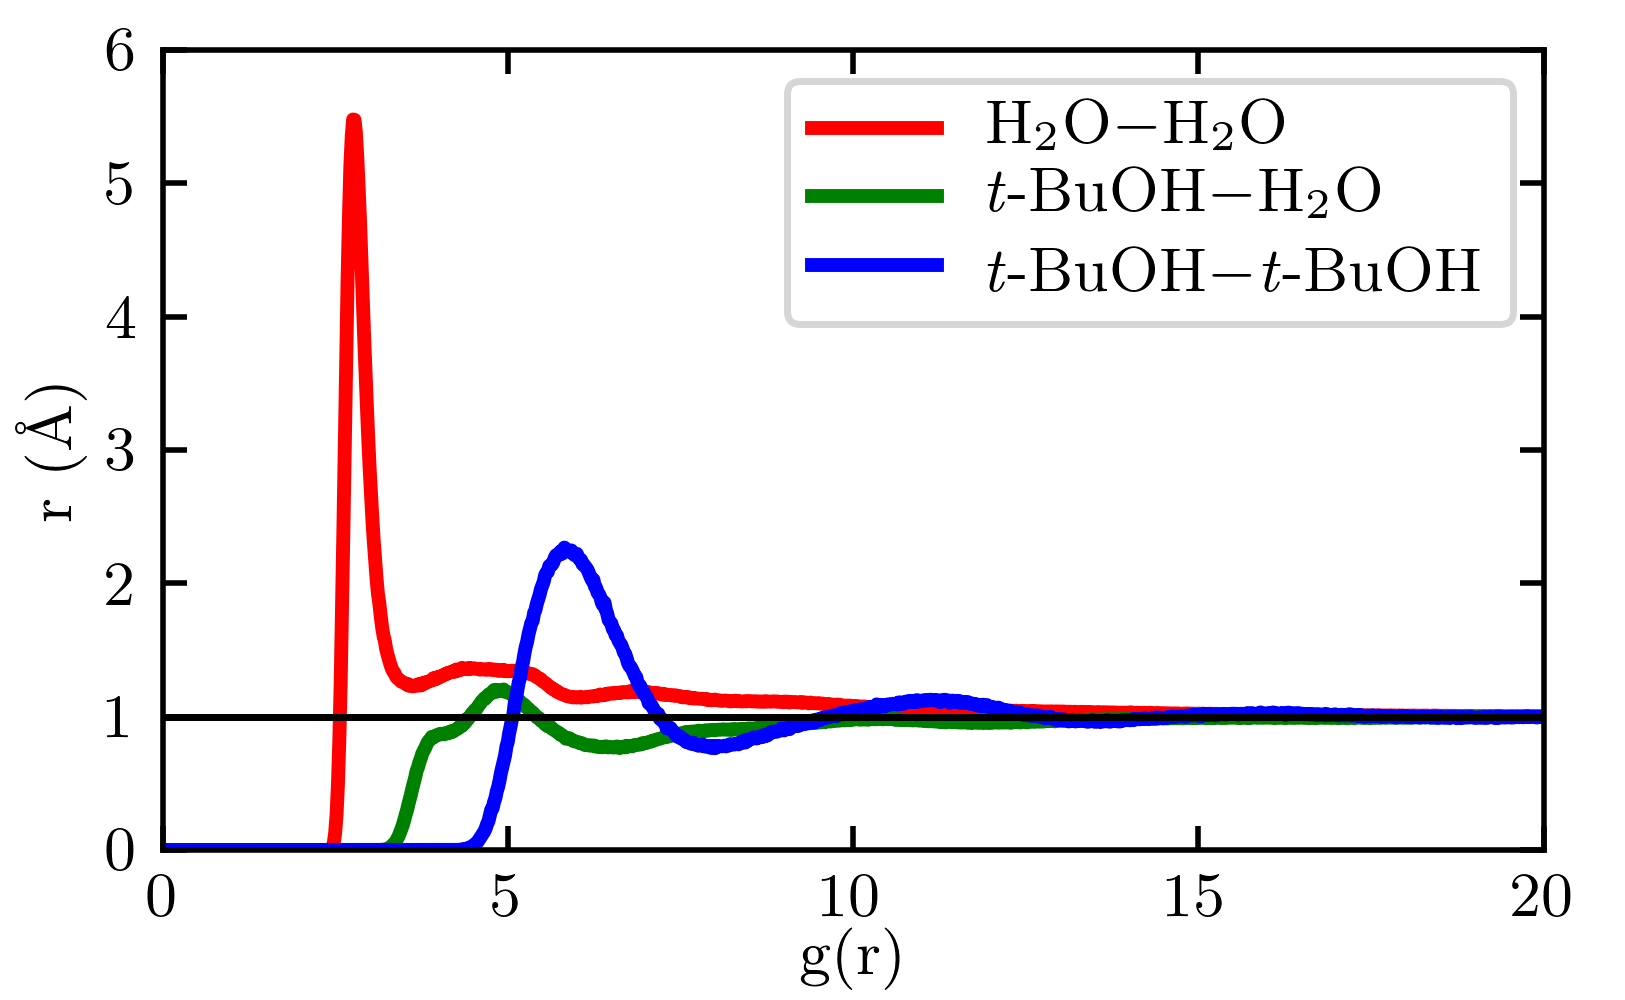
\includegraphics[width=\single]{figures-helix/rdfs.png}
    \caption[Pair correlation functions between solvent molecules in a binary mixture]{
        Pair correlation functions matched those reported in ref \citenum{DiPierro2015} indicating that the \tba{} parameters were implemented correctly for Gromacs. 
        Red: Pair correlation function between the oxygen atoms of water molecules and the oxygen atoms of other water molecules. 
        Green: Pair correlation function between the central carbon of \tba{} and the oxygen atoms of water molecules. 
        Blue: Pair correlation function between the central carbon atom of \tba{} and the central carbon atoms of other \tba{} molecules. 
    }
    \label{fig:helix-rdfs}
\end{figure}

\begin{figure}
    \center
    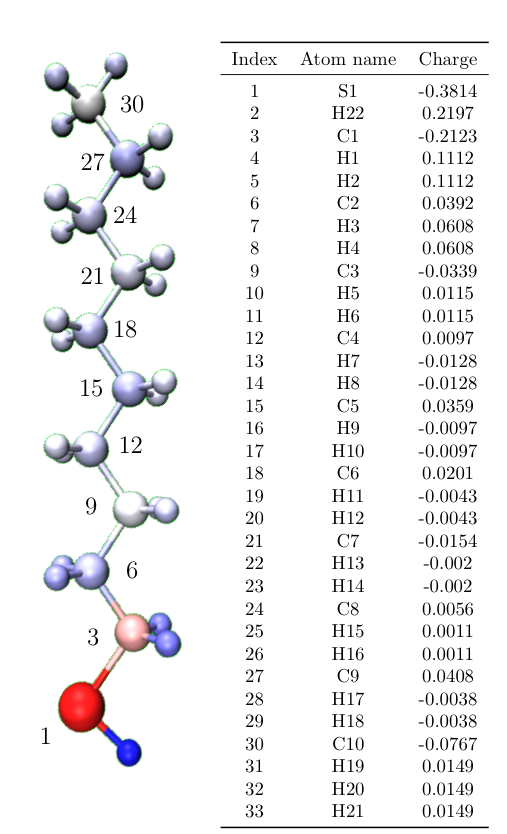
\includegraphics[width=\single]{figures-helix/charge_figure.png}
    \caption[Derived partial charges of decanethiol]{
        Derived partial charges for the decanethiol molecule used in the SAM. 
        The atoms are colored by charge, where red represents a more negatively charged atom, and blue represents a more positively charged atom. 
        The heavy atoms are indexed and the partial charges can be found in the table. 
        Hydrogens appear under the heavy atom to which they are bound.
    }
    \label{fig:helix-charges}
\end{figure}

\subsection{Water simulation}

The peptide was minimized in vacuum using the steepest descent algorithm and solvated in a 7.6 nm cubic box of TIP3P water \cite{Jorgensen1983}. 
The solvated system was then minimized using the steepest descent algorithm, heated to 300 K under the NVT ensemble for 50 ps, and equilibrated under the NPT ensemble at 1 atm for 100 ps, each with heavy atom restraints on the peptide atoms. 
This equilibrated system was used to begin the simulation of the folded peptide in water. 

\subsection{Binary mixture simulation}

A 2:1 (v/v) \tba{}:\ce{H2O} mixture was created by distributing 1831 molecules of united atom \tba{} (Figure \ref{fig:helix-tba}) and 4862 TIP3P water molecules in a 7.6 nm cubic box. 
This box was energy minimized using the steepest descent algorithm, heated to 300 K under the NVT ensemble for 50 ps, and equilibrated under the NPT ensemble at 1 atm for 100 ps. 
The starting peptide was then energy minimized using the steepest descent algorithm and placed inside the equilibrated solvent mixture. 
The system was again energy minimized using the steepest descent algorithm, then heated to 300 K under the NVT ensemble for 50 ps, and equilibrated under the NPT ensemble at 1 atm for 100 ps. 
This equilibrated system was used to begin the simulation of the folded peptide in \tbawat{}. 

\subsection{SAM surface simulation}

A SAM was built by placing decanethiol molecules in a hexagonal packing arrangement according to Ulman et al.\cite{Ulman1989}, with an intermolecular spacing of 4.97 \si{\angstrom}, using an in-house Python code and the gmx insert-molecules module. 
To simulate bonds from the decanethiols to the Au surface, which was not present in the simulations, the sulfur atoms of the decanethiols were restrained to their horizontal $x$-$y$ plane with a harmonic restraint of $2\cdot10^3$ kJ mol$^{-1}$ nm$^{-2}$. 
The SAM was energy minimized using the steepest descent algorithm, and then heated to 300 K under the NVT ensemble for 50 ps. 
Separately, the starting peptide was energy minimized using the steepest descent algorithm and solvated in a 6.0 nm $\times$ 7.0 nm $\times$ 6.0 nm box of TIP3P water. 
The $x$, $y$ dimensions were matched to the dimensions of the decanethiol layer. 
The $z$ dimension was chosen to ensure that the peptide cannot interact with the bottom of the decanethiol layer across the periodic boundary. 
The solvated system was then energy minimized using the steepest decent algorithm, headed to 300 K under the NVT ensemble for 50 ps, and equilibrated under a semi-isotropic NPT ensemble at 1 atm for 100 ps with volumetric fluctuations restricted to the $z$ dimension, each with heavy atom restraints on the peptide. 

The solvated system and the SAM were then combined so that the peptide was 6.822 \si{\angstrom} away from the top of the SAM. 
Again, in order to mitigate the effect of the sulfur layer of the SAM across the $z$-dimension of the periodic boundary, the size of the water layer in between the peptide and the neighboring sulfur layer was chosen to be much larger than the electrostatic cutoff of the simulations. 
An illustration of this system is shown in Figure \ref{fig:helix-system}. 
The azido linker group, which covalently bonds the peptide to the SAM surface in experiment, was approximated with a harmonic restraint of 103 kJ mol$^{-1}$ nm$^{-2}$ and equilibrium bond length of 6.822 \si{\angstrom} between the Gly C\textalpha{} atoms and the C10 of the nearest decanethiol molecule. 
This distance, which is illustrated in Figure \ref{fig:helix-linker}, was chosen based on a DFT energy minimized structure at the wB97X-D/6-311$+$G** level using the Spartan QM software suite\cite{Shao2006}.   
The system was again energy minimized using the steepest descent algorithm, heated to 300 K under the NVT ensemble for 50 ps, then equilibrated under the NPT ensemble at 1 atm for 100 ps with volumetric fluctuations restricted to the $z$ dimension. 
The harmonic restraints binding the peptide to the SAM were removed for the production simulation, unless otherwise noted.

\begin{figure}
    \center
    \includegraphics[width=\single]{figures-helix/system3.png}
    \caption[Starting configuration of \pep{} on the surface of a SAM]{
        A snapshot of the starting configuration for \pep{} on the surface of a decanethiol SAM. 
        The peptide (cyan ribbon) is shown in the folded starting configuration, with lysine residues (red) facing up away from the SAM and leucine residues (gray) facing down toward the SAM. 
        The yellow, cyan, and white spheres are the sulfur, carbon, and hydrogen atoms, respectively, of the decanethiol molecules. 
        The small red and white sticks represent water molecules. 
        The green spheres in solution represent chloride ions. 
    }
    \label{fig:helix-system}
\end{figure}

\begin{figure}
    \center
    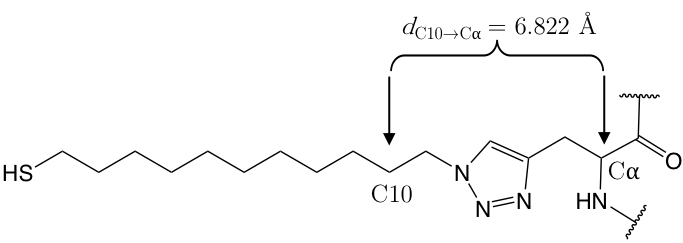
\includegraphics[width=4.5in]{figures-helix/Linker_figure.png}
    \caption[The product of the Huisgen cycloaddition]{
        The product of the Huisgen cycloaddition. 
        The long alkane chain sits in a SAM of decanethiols, and the sulfur atom is covalently attached to a Au(111) surface. 
        The C\textalpha{} is from one of the two propargylglycine residues of \pep{}. 
        For simplicity, we have replaced the propargylglycine with a glycine residue in the simulations. 
        The C\textalpha{} of the glycine residues were harmonically restrained to the nearest C10 on the SAM at a distance of 6.822 \si{\angstrom} (the distance in the DFT geometry optimized structure) during the annealing process and were kept or removed for the production simulations, as discussed in the main text.
    }
    \label{fig:helix-linker}
\end{figure}

\subsection{Simulated annealing}\label{helix-anneal}

In order to prepare the unfolded structure in each of the solvent environments, the heavy atom restraints on the peptide were removed. 
Using the Berendsen thermostat, the systems were coupled to a heat bath that increased by 12 K every 10 ps for 500 ps. 
The systems were equilibrated at 900 K for 100 ps, and then coupled to a heat bath that decreased by 12 K every 10 ps for 500 ps. 
A representative temperature curve from this annealing process is shown in Figure \ref{fig:helix-anneal}A. 
For the simulations that included a SAM layer, harmonic restraints of 107 kJ mol$^{-1}$ nm$^{-2}$ were applied during the annealing process to the heavy atoms of the SAM to keep the layer intact. 
Each system was visually inspected to confirm the peptide had unfolded during the annealing process. 
The DSSP structural assignments (see below) showed complete unfolding for each peptide; 
these are shown in Figures \ref{fig:helix-anneal}B,C,D for the peptide in water, in \tbawat{}, and on the SAM surface respectively.

\begin{figure}
    \center
    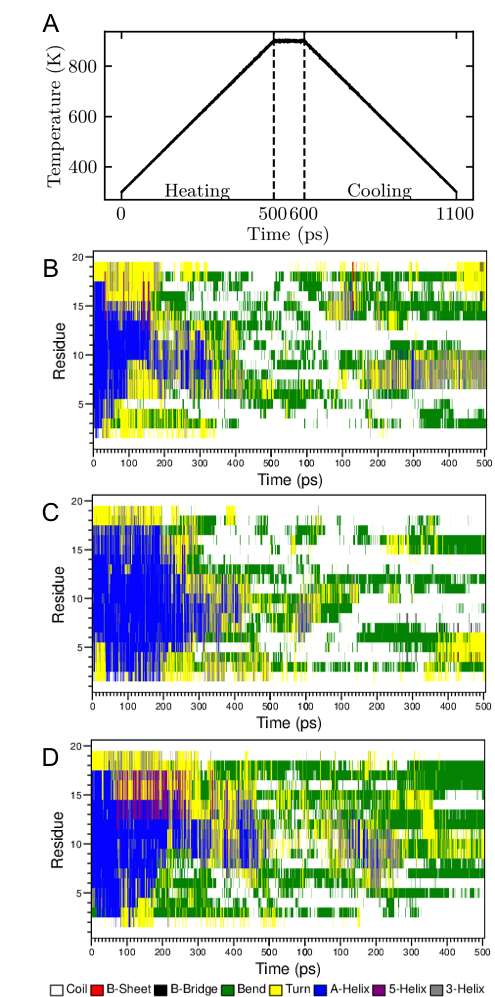
\includegraphics[width=2.75in]{figures-helix/unfolding.png}
    \caption[Annealing procedure used to unfold \pep{}]{
        A: Temperature curve for the simulated annealing process used to generate the unfolded structures. 
        The dashed lines separate the stages of the annealing process. 
        B, C, and D: DSSP structural assignments for \pep{} in water, in \tbawat{} and on the SAM, respectively, during the annealing process. 
        Note that all of the initial structure is lost in each system in the first 500 ps (the heating stage). 
        The final structure from the annealing process was used to initiate the simulations of the unfolded peptide in each solvent environment.
    }
    \label{fig:helix-anneal}
\end{figure}

\subsection{Production simulations and analyses}

For each of the three environments, a production simulation was run from a folded structure of the peptide and from an unfolded structure of the peptide, resulting in six simulations. 
Simulations were run for 1.25 \textmu{}s each, using a 2 fs time step and a stochastic integrator. Particle-mesh-Ewald (PME) electrostatics was implemented with a Coulombic cutoff of 10 \si{\angstrom}. 
Van der Waals (VDW) interactions were cut off at 10 \si{\angstrom}. 
Snapshots were recorded every 4 ps during simulations.

Structural assignments were calculated using the DSSP algorithm (discussed further below)\cite{Kabsch1983, Joosten2011} through the gmx do\_dssp interface. 
Radii of gyration ($R_g$), RMSDs, pair correlation functions, and free energy surfaces were calculated using gmx modules. 
Cluster analyses were performed using the Gromos algorithm\cite{Daura1999} and the gmx cluster module with a cutoff of 2.5 \si{\angstrom} backbone RMSD between clusters. 
CD line spectra were computed at every 100 ps using the DichroCalc portal\cite{Bulheller2009, Jasim2018} using both the Hirst basis set\cite{Hirst1998, Besley1999} and the Woody basis set\cite{Woody1999}, both with backbone transfer transitions. 
All other options were left as default. 
The line spectra were then convoluted with Gaussian functions to produce continuous spectra, as discussed in the main text.

%%%%%%%%%%%%%%%%%%%%%%%%%%%%%%%%%%%%%%%%%%%%%%%%%%%%%%%%%%%%%%%%
%%%%%%%%%%%%%%%%%%%%%%%%%%%%%%%%%%%%%%%%%%%%%%%%%%%%%%%%%%%%%%%%
\section{Results}\index{helix-results}
%%%%%%%%%%%%%%%%%%%%%%%%%%%%%%%%%%%%%%%%%%%%%%%%%%%%%%%%%%%%%%%%
%%%%%%%%%%%%%%%%%%%%%%%%%%%%%%%%%%%%%%%%%%%%%%%%%%%%%%%%%%%%%%%%

In order to successfully and reliably integrate proteins onto inorganic materials, it is necessary to attach them reproducibly to surfaces and substrates with the appropriate structure, orientation, and chemical environment for function. 
Understanding any conformational changes that are imparted by the surface material is critical to this goal but remains a longstanding challenge \cite{Hlady1996, Castner2002, Latour2005biomaterials}.
In order to test if the generally applicable force field (OPLS-AA) is reliable at a surface for the \pep{} peptide and can capture conformational changes that are potentially critical to its ability to noncovalently immobilize proteins at a surface in a biomimetic fashion, we used MD simulations to investigate the known solvent-induced and surface-induced structural changes of the peptide.

\subsection{Conformational differences and sampling}

Previously, CD spectra (Figure \ref{fig:helix-cd_spectra}) had indicated that \pep{} was unfolded in aqueous solution, partially helical in \tbawat{}, and significantly helical on the surface of a decanethiol SAM \cite{Gallardo2012}. 
To avoid biasing the simulations by starting structure, we ran two separate trajectories for each of the three solvent environments: one from a folded \textalpha{}-helix and one from an unfolded, disordered structure. 
We then ran MD simulations on each of the six systems for 1.25 \textmu{}s. 
At each frame of the trajectories we calculated the peptide secondary structure using the DSSP algorithm\cite{Kabsch1983, Joosten2011}, which categorizes residues into eight classifications based on estimated hydrogen bonding energies: \textalpha{}-helix, $3_{10}$-helix, \textpi{}-helix, turn, \textbeta{}-sheet, \textbeta{}-bridge, bend, and coil. 
The total breakdown of secondary structure by residue is plotted against simulation time for each of the six trajectories in Figure \ref{fig:helix-dssp}. 
Since we are interested in a more broadly defined structural change, we grouped each of these secondary structures into four larger categories: 1) helical (\textalpha{}-helix, $3_{10}$-helix, or \textpi{}-helix); 2) turn; 3) strand (\textbeta{}-sheet, \textbeta{}-bridge, or bend); and 4) unfolded (coil). 
The fraction of residues in each of these categories was calculated, binned to smooth the data, and plotted in Figure \ref{fig:helix-conf_fracs}, where dark blue represents the fraction of residues in a helical conformation, light blue represents the fraction of residues in a turn, green represents the fraction of residues in a strand, and red represents the fraction of residues in an unfolded conformation. 
Each category is offset on the $y$-axis to avoid overlap and will be referred to hereafter as the stacked ``conformational fractions.'' 

\begin{figure}
    \center
    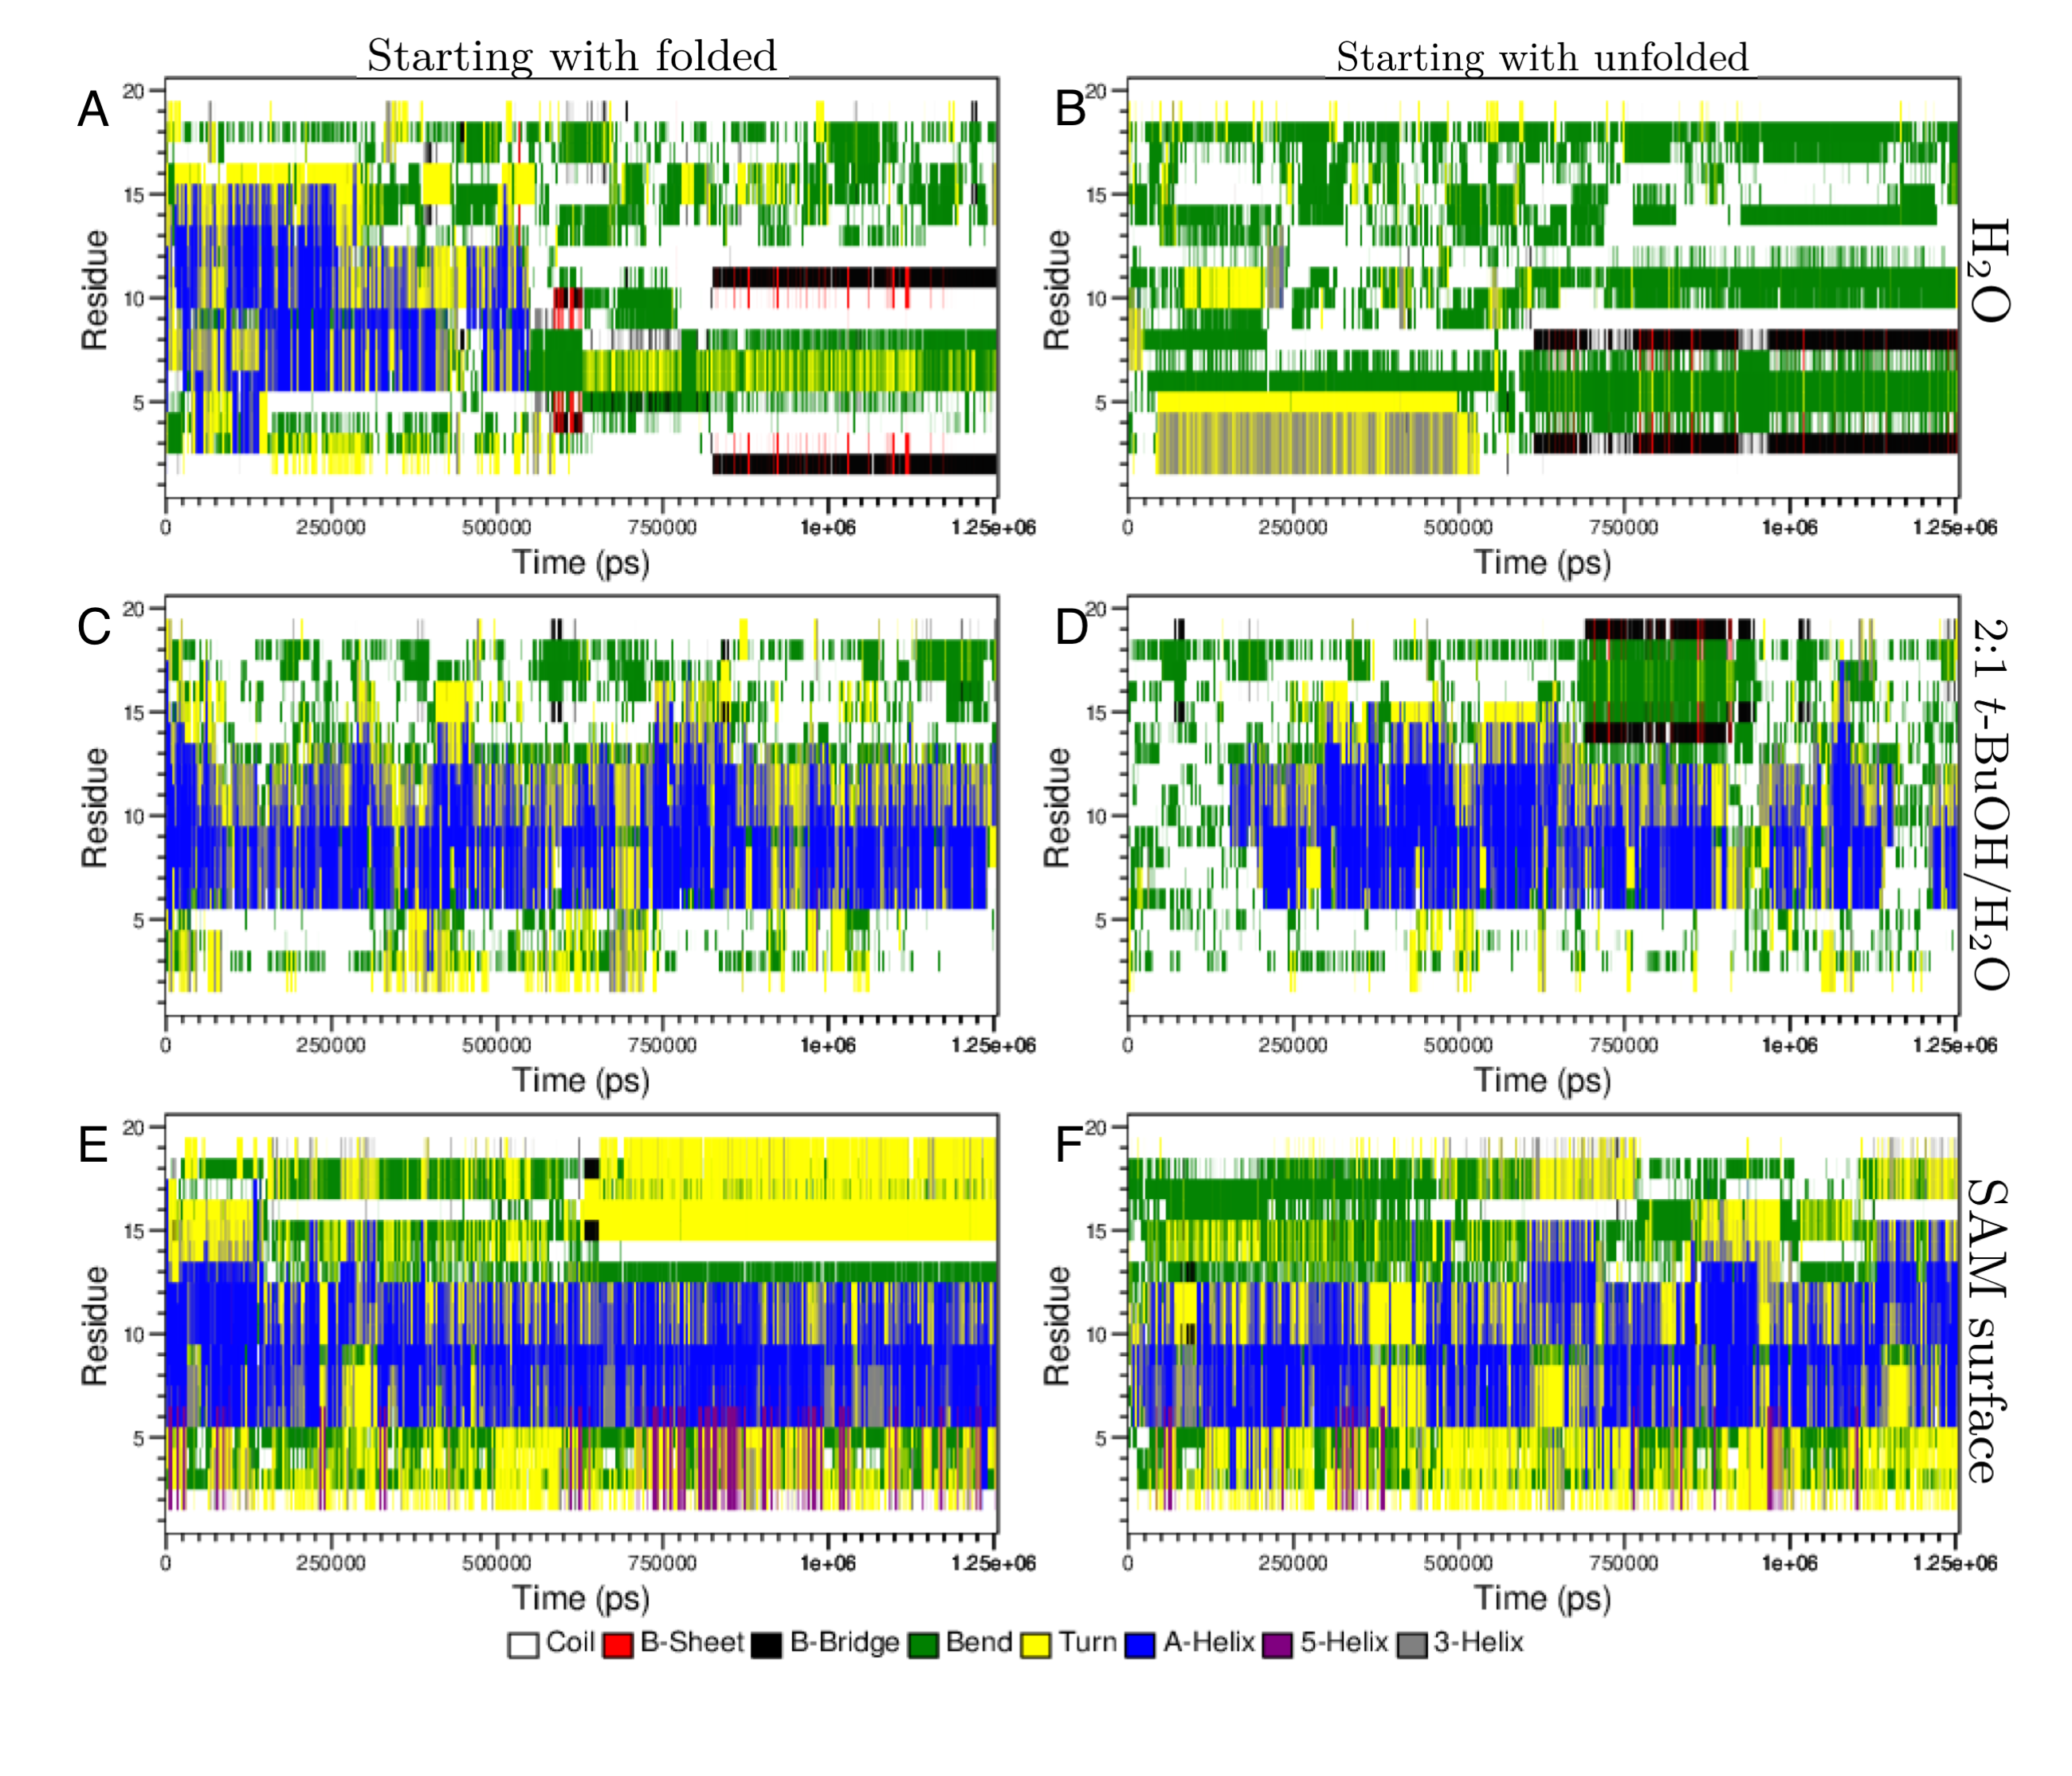
\includegraphics[width=\double]{figures-helix/dssp.png}
    \caption[DSSP structural assignments by residue for \pep{}]{
        DSSP structural assignments by residue for simulations of \pep{}. 
        A, C, E: \pep{} began the simulation in an \textalpha{}-helical conformation. 
        B, D, F: \pep{} began the simulation unfolded.
        A, B: the peptide was dissolved in water. 
        C, D: the peptide was dissolved in \tbawat{}. 
        E, F: the peptide was on the surface of a SAM dissolved in water.
    }
    \label{fig:helix-dssp}
\end{figure}

\begin{figure}
    \center
    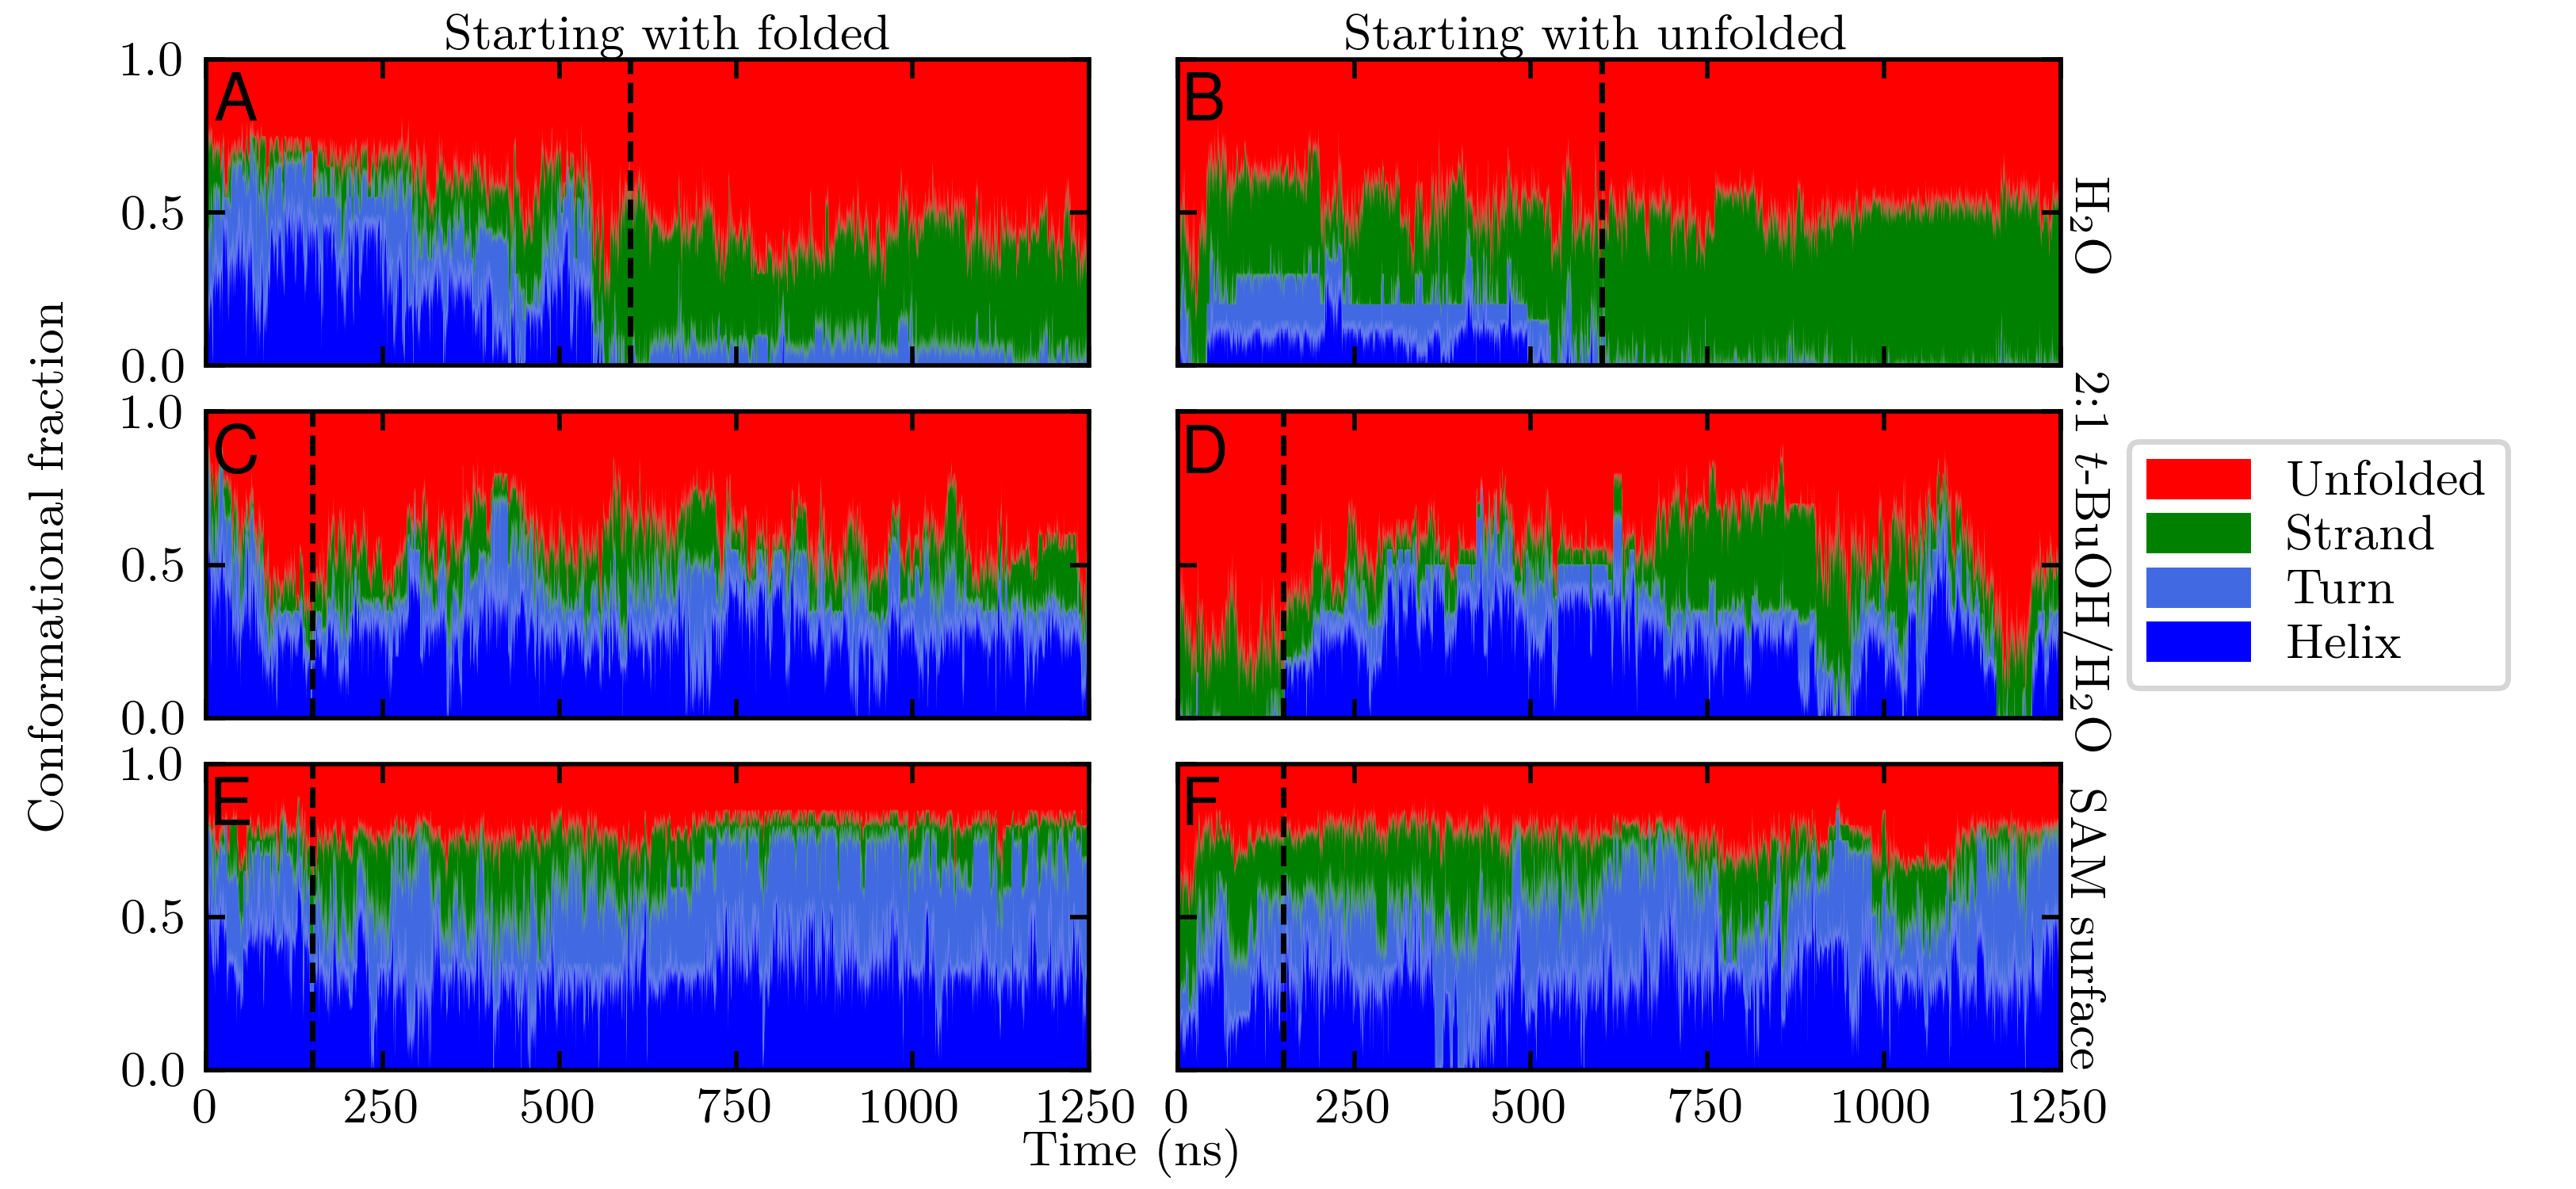
\includegraphics[width=\double]{figures-helix/combined_helicity.png}
    \caption[Stacked conformational fractions of \pep{} in three different solvent environments]{
        Stacked conformational fractions of \pep{} in three different solvent environments. 
        Blue: fraction of residues assigned to a helical secondary structure. 
        Light blue: fraction of residues assigned to a turn secondary structure. 
        Green: fraction of residues assigned to a strand secondary structure. 
        Red: fraction of residues assigned to unfolded secondary structure. 
        A, C, E: \pep{} began the simulation in a \textalpha{}-helical conformation. 
        B, D, F: \pep{} began the simulation unfolded. 
        A, B: the peptide was dissolved in water. 
        C, D: the peptide was dissolved in \tbawat{}. 
        E, F: the peptide was on the surface of a SAM dissolved in water. 
        The black dashed lines represent the determined equilibration time for each simulation. 
        The data after this mark was averaged and is presented in Table \ref{tbl:helix-frac_bestsel}.
    }
    \label{fig:helix-conf_fracs}
\end{figure}

When the simulation of \pep{} in water was initiated from a folded helical conformation (Figure \ref{fig:helix-conf_fracs}A), the peptide began the simulation with high helical character (0.70 helical and 0.15 turn). 
For the first 600 ns, the helical character of the peptide slowly decreased, resulting in an unfolded peptide. 
After this time, the peptide adopted significant strand character (average of 0.36 strand), which was retained through the duration of the simulation. 
Figure \ref{fig:helix-dssp}A shows that the strand character mostly occurred at the N-terminal region (residues 2-11), and the rest of the peptide was unstructured. 
Starting from an unfolded conformation in water (Figure \ref{fig:helix-conf_fracs}B), the peptide began with little helical or turn character. 
For the first 600 ns, the peptide sampled conformations with some helical character and some strand character, but eventually adopted a conformation with no helical character and high strand character (average of 0.50 strand). 
Figure \ref{fig:helix-dssp}B shows that the strand character occurred again at the N-terminal region (residues 3-8), and the rest of the peptide was unstructured. 
Despite starting from very different conformations, both simulations of \pep{} in water displayed similar secondary structure, with strand character at the N-terminal region and the rest of the peptide unstructured. 
Because 600 ns elapsed before \pep{} adopted similar secondary structure in both simulations, 600 ns was taken to be the equilibration time for both of these simulations, and the first 600 ns of these trajectories was not included in the analyses that follow for \pep{} in water.

When the simulation of \pep{} in \tbawat{} was started from a folded helical conformation (Figure \ref{fig:helix-dssp}C), the peptide began the simulation with significant helical character (0.80 helical and 0.10 turn). 
Over the first 150 ns, the helical fraction decreased rapidly to ~0.3 and the unfolded character increased to ~0.5. 
This helicity was then retained for the duration of the simulation. 
Figure \ref{fig:helix-dssp}C shows that the helicity was lost at residues 1-5 and 15-20 (the two terminal regions), and the middle region of the peptide (residues 6-14) remained helical. 
Starting from an unfolded conformation in \tbawat{} (Figure \ref{fig:helix-conf_fracs}D), the peptide began the simulation with little helical character. 
For the first 150 ns, the peptide sampled configurations with mostly unfolded character, and after this time the peptide primarily sampled helical configurations that were retained through the duration of the simulation. 
Figure \ref{fig:helix-dssp}D shows that the helical character was again in the middle region of the peptide (residues 6-14), and the unfolded character dominated the two terminal regions (residues 1-5 and 15-20). 
Again, despite starting from very different conformations, both simulations of \pep{} in \tbawat{} displayed similar secondary structure. 
Because 150 ns elapsed before the peptide attained this secondary structure, 150 ns was taken to be the equilibration time for both of these simulations, and the first 150 ns of these trajectories was not included in the analyses that follow for \pep{} in \tbawat{}. 

Finally, when the simulation of \pep{} on the surface of a SAM was started from a folded helical conformation (Figure \ref{fig:helix-conf_fracs}E), the peptide retained its helical and turn structure throughout the entire 1.25 \textmu{}s simulation. 
Figure \ref{fig:helix-dssp}E shows that the helicity again occured in the middle region of the peptide (residues 6-14), and that the two terminal regions (residues 1-5 and 15-20) were mostly classified as ``turn.'' 
Starting from an unfolded structure on the surface of the SAM (Figure \ref{fig:helix-conf_fracs}F), the peptide acquired significant helical and turn character within 50 ns that persisted for the duration of the simulation. 
Figure \ref{fig:helix-dssp}F shows that the helical structure was again attributed to the middle region of the peptide (residues 6-14), and that the two termini regions contained mostly turn character. 
As for the simulations of \pep{} in solution, despite starting from very different conformations, both simulations of \pep{} on the surface of a SAM displayed similar secondary structure, demonstrating the strong bias towards helical conformations for \pep{} on the SAM surface. 
Because the equilibration time was not as visually clear from Figures \ref{fig:helix-conf_fracs}E,F as for the solvated peptides, 150 ns was taken to be the equilibration time to be consistent with the simulations in \tba{}; 
the first 150 ns of these trajectories was not included in the analyses that follow for \pep{} on the surface of the SAM.

As with any biomolecular simulation, the convergence of the trajectories to a consistent result must be carefully considered. 
While convergence is difficult to achieve without advanced sampling techniques, particularly since the nucleation time of helices is often hundreds of nanoseconds, we have chosen to mitigate the bias from the starting conformation by starting the simulations from opposite ends of the folding reaction coordinate. 
Since the two simulations in each environment reached similar structures from such different starting points, it is unlikely that the result of the simulations will change with additional sampling time and likely that unsampled conformations are similar to those already observed. 
While the stacked conformational fractions (Figure \ref{fig:helix-conf_fracs}) clearly demonstrate similar secondary structure between the two trajectories for each solvent, many different structures can give rise to the same secondary structure assignment. 
We therefore also examined whether the folded and unfolded peptides reached similar configurational space by calculating the backbone RMSD from the helical structure and the radius of gyration ($R_g$) of the peptide. 
Figure \ref{fig:helix-rgyr_v_rmsd} shows the movement of each peptide along this configuration space over the course of the trajectories, where each point represents a 100 ps window average. 
In water, both trajectories heavily sampled the configuration space with a $R_g$ of 9-11 \si{\angstrom} and a backbone RMSD of 8-9 \si{\angstrom} away from the perfectly folded \textalpha{}-helix. 
In \tbawat{}, both trajectories sampled a configuration space with a $R_g$ of 11-12 \si{\angstrom} and were closer to a perfectly folded \textalpha{}-helix with a backbone RMSD of 4-6 \si{\angstrom}. 
Finally, on the surface of the SAM, both trajectories sampled a configuration space with a $R_g$ of 8-11 \si{\angstrom} and were only 1.5–5 \si{\angstrom} backbone RMSD from the perfectly folded \textalpha{}-helix. 
The RMSD data demonstrated that the helical character of \pep{} increased from water to \tbawat{}, and then further increased when interacting with the surface of the SAM, consistent with our expectation from the experimental CD spectra in Figure \ref{fig:helix-cd_spectra}. 
Further, each of these sets of simulations reached similar configuration space despite beginning from different starting structures, indicating that we have mitigated the bias of our starting structure towards our results.

\begin{figure}
    \center
    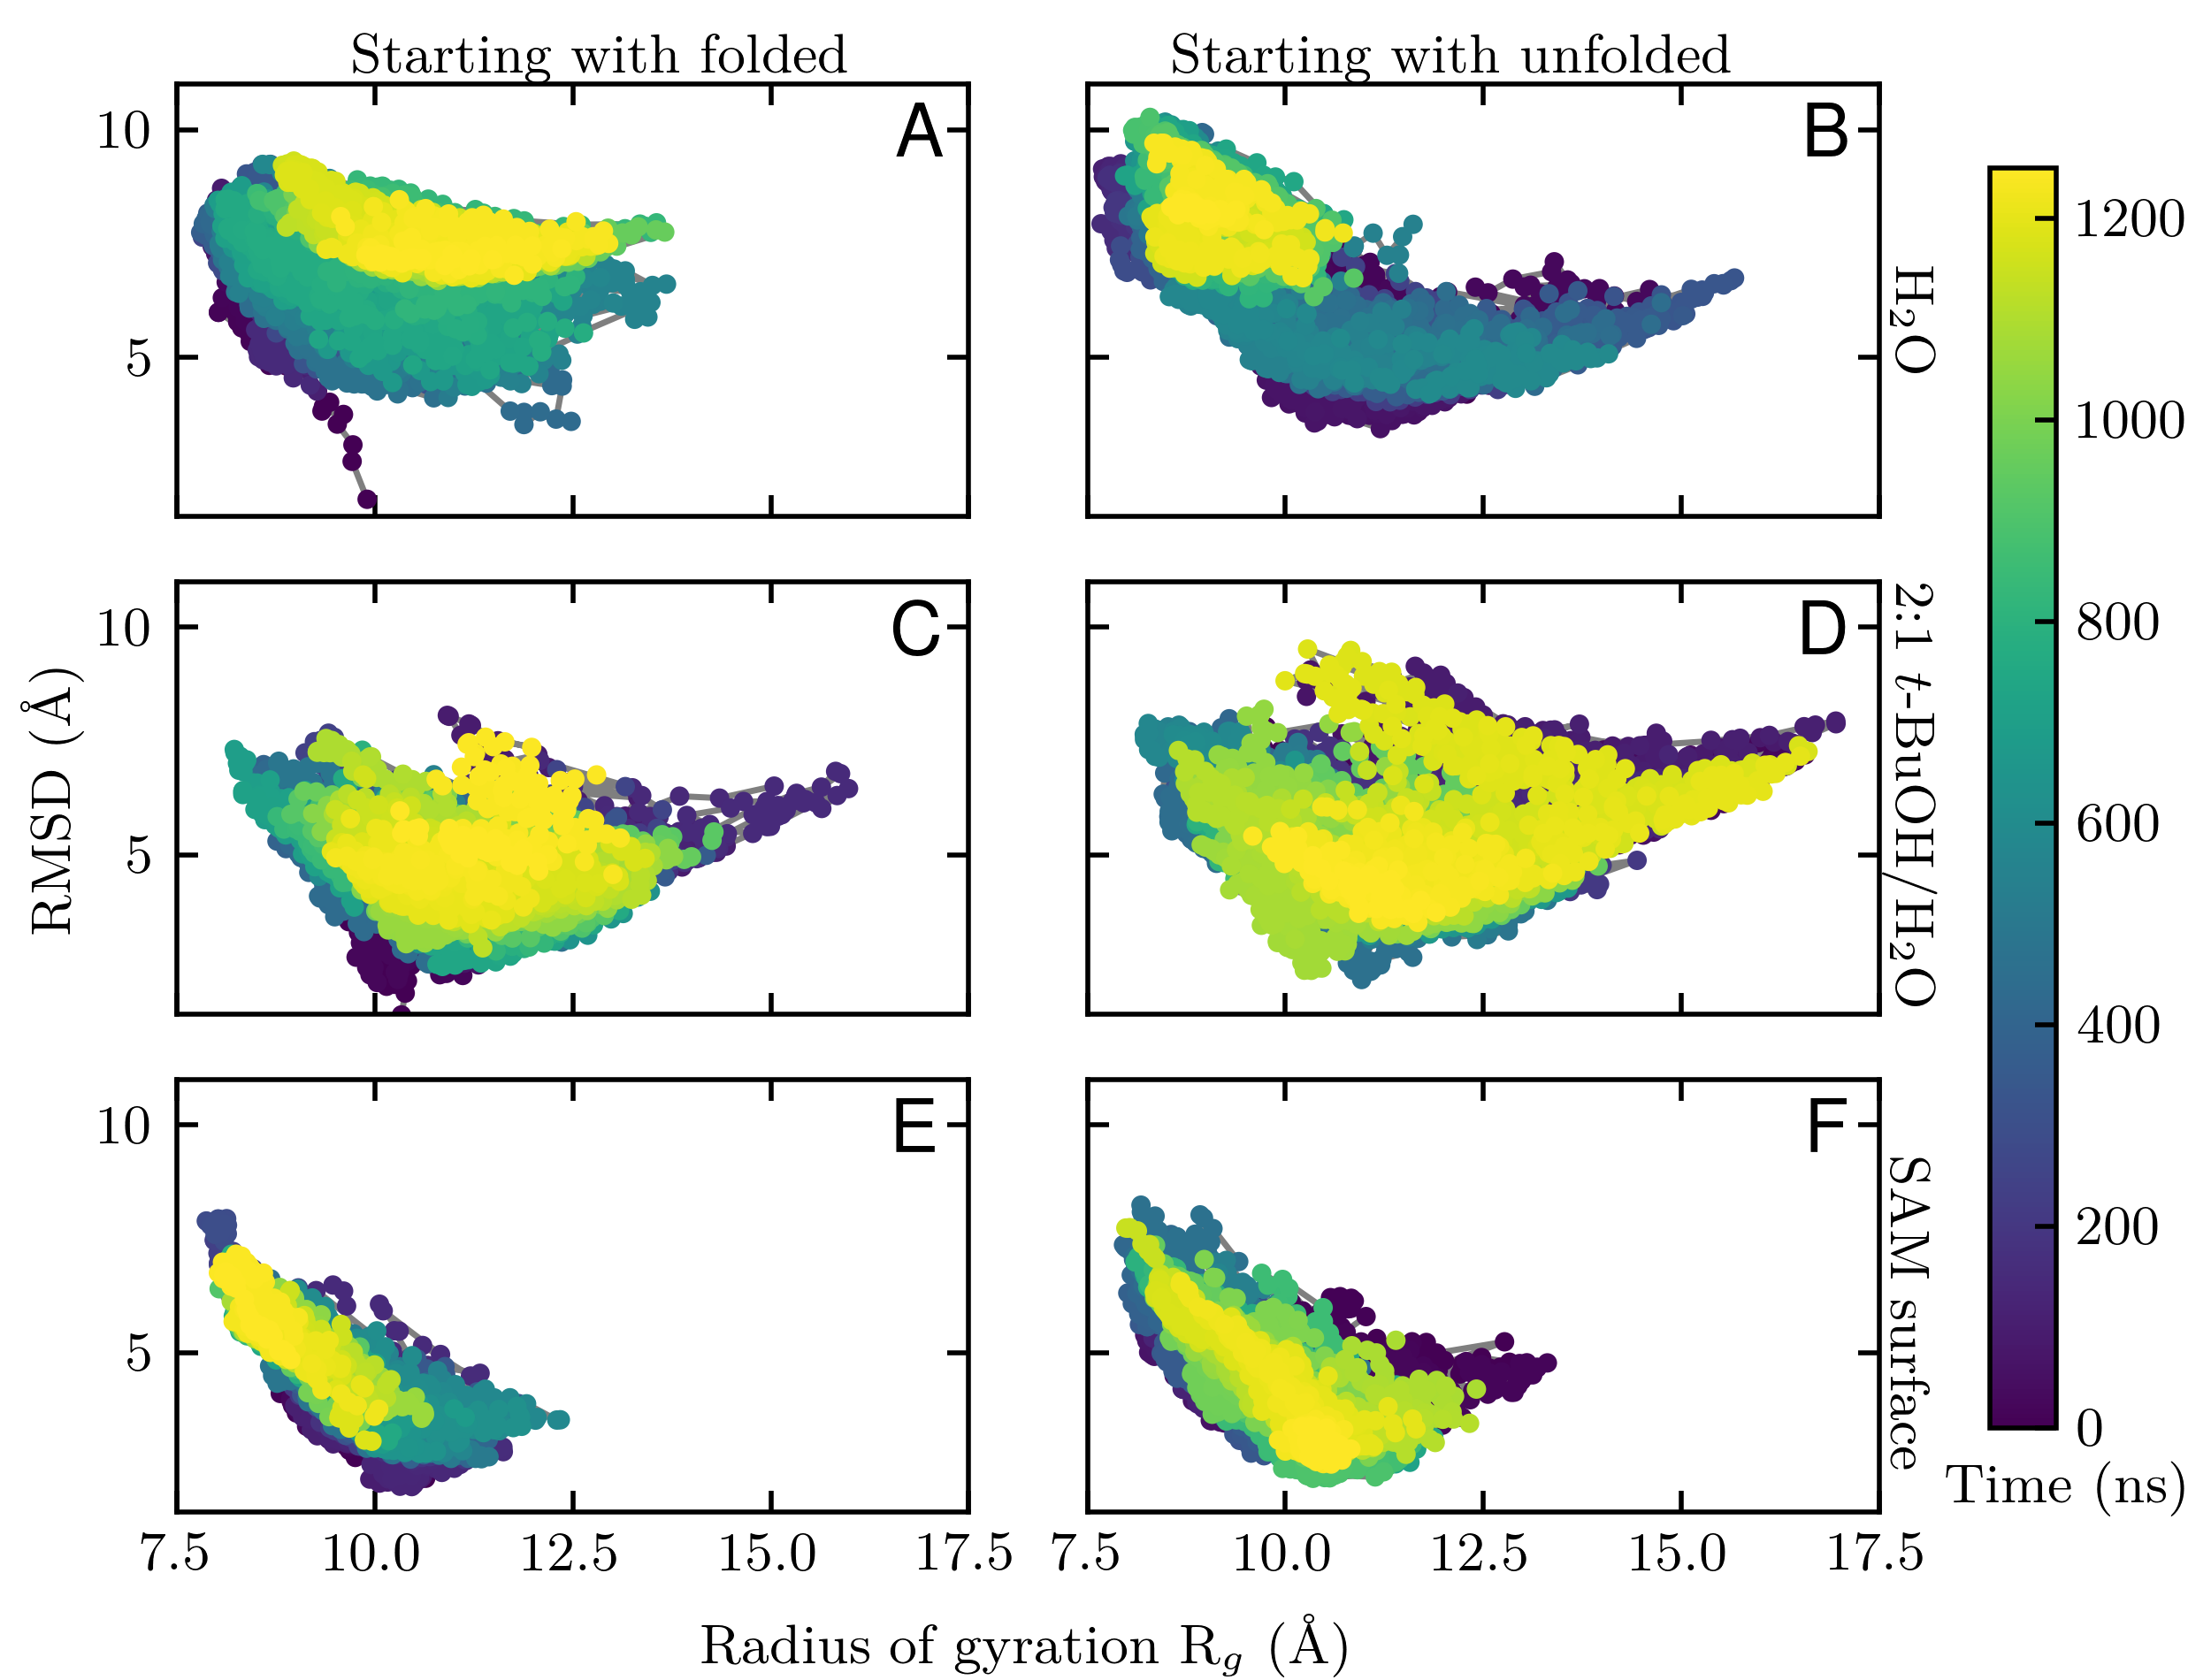
\includegraphics[width=\double]{figures-helix/combined_rgyr_v_rmsd.png}
    \caption[Conformational space sampled by \pep{} in three different solvents]{
        Conformational space sampled by \pep{} in six simulations. 
        On the $x$-axis is the radius of gyration of the protein. 
        On the $y$-axis is the backbone RMSD away from a perfectly folded \textalpha{}-helix. 
        Each point represents a 100 ps average and is colored by its time. 
        A, C, E: \pep{} began the simulation in an \textalpha{}-helical conformation. 
        B, D, F: \pep{} began the simulation unfolded. 
        A, B: the peptide was dissolved in water. 
        C, D: the peptide was dissolved in \tbawat{}. 
        E, F: the peptide was on the surface of a SAM dissolved in water.
    }
    \label{fig:helix-rgyr_v_rmsd}
\end{figure}

\subsection{Free energy analysis of folding}

In~ order~ to~ further~ investigate~ the~ preferential~ folding~ of~ \pep{}~ in~ \tbawat{} and on the surface of a SAM, we calculated the 2D free energy surface sampled in each environment. 
From the combined ensemble (the trajectory from the folded conformation and from the unfolded conformation, excluding snapshots prior to the equilibration times), we binned the calculated backbone RMSD from the \textalpha{}-helical conformation and $R_g$ (from Figure \ref{fig:helix-rgyr_v_rmsd}) and inverted the histogram according to eq \ref{eq:helix-boltz} using the gmx sham module:
\begin{equation}
    \Delta G = -k_B \ln(P)
    \label{eq:helix-boltz}
\end{equation}
where $\Delta G$ is the relative free energy of the bin, $k_B$ is the Boltzmann constant, and $P$ is the relative probability of the bin taken from the histogram. 
The calculated free energy surfaces are shown in Figures \ref{fig:helix-free_cluster}A-C, where $\Delta G$ of the unsampled regions were defined to be zero. 
The free energy surface (Figure \ref{fig:helix-free_cluster}A) of \pep{} in water displayed a free energy minimum ($\Delta G = -21.4$ kJ mol$^{-1}$) at high RMSD and low $R_g$, consistent with compact, non-helical conformations. 
In \tbawat{}, the free energy surface (Figure \ref{fig:helix-free_cluster}B) was shallower and more diffuse with a less distinct minimum ($\Delta G = -18.7$ kJ mol$^{-1}$), indicating partial destabilization of the most probable conformations. 
Conformations with high $R_g$ and low RMSD, consistent with extended, helical structures, were more stabilized in \tbawat{} than in water. 
On the surface of the SAM, the free energy surface (Figure \ref{fig:helix-free_cluster}C) favored conformations with low $R_g$ and low RMSD, consistent with compact, helical conformations. 
The minimum ($\Delta G = -22.5$ kJ mol$^{-1}$) had slightly higher RMSD to that in \tbawat{} with much lower $R_g$, and another minimum was apparent at lower RMSD and similar $R_g$ to that in \tbawat{}. 
Together, these results demonstrate that water stabilizes compact, non-helical conformations of \pep{}, \tbawat{} weakly stabilizes extended, helical conformations, and the SAM surface strongly stabilizes compact, helical conformations.

\begin{figure}
    \center
    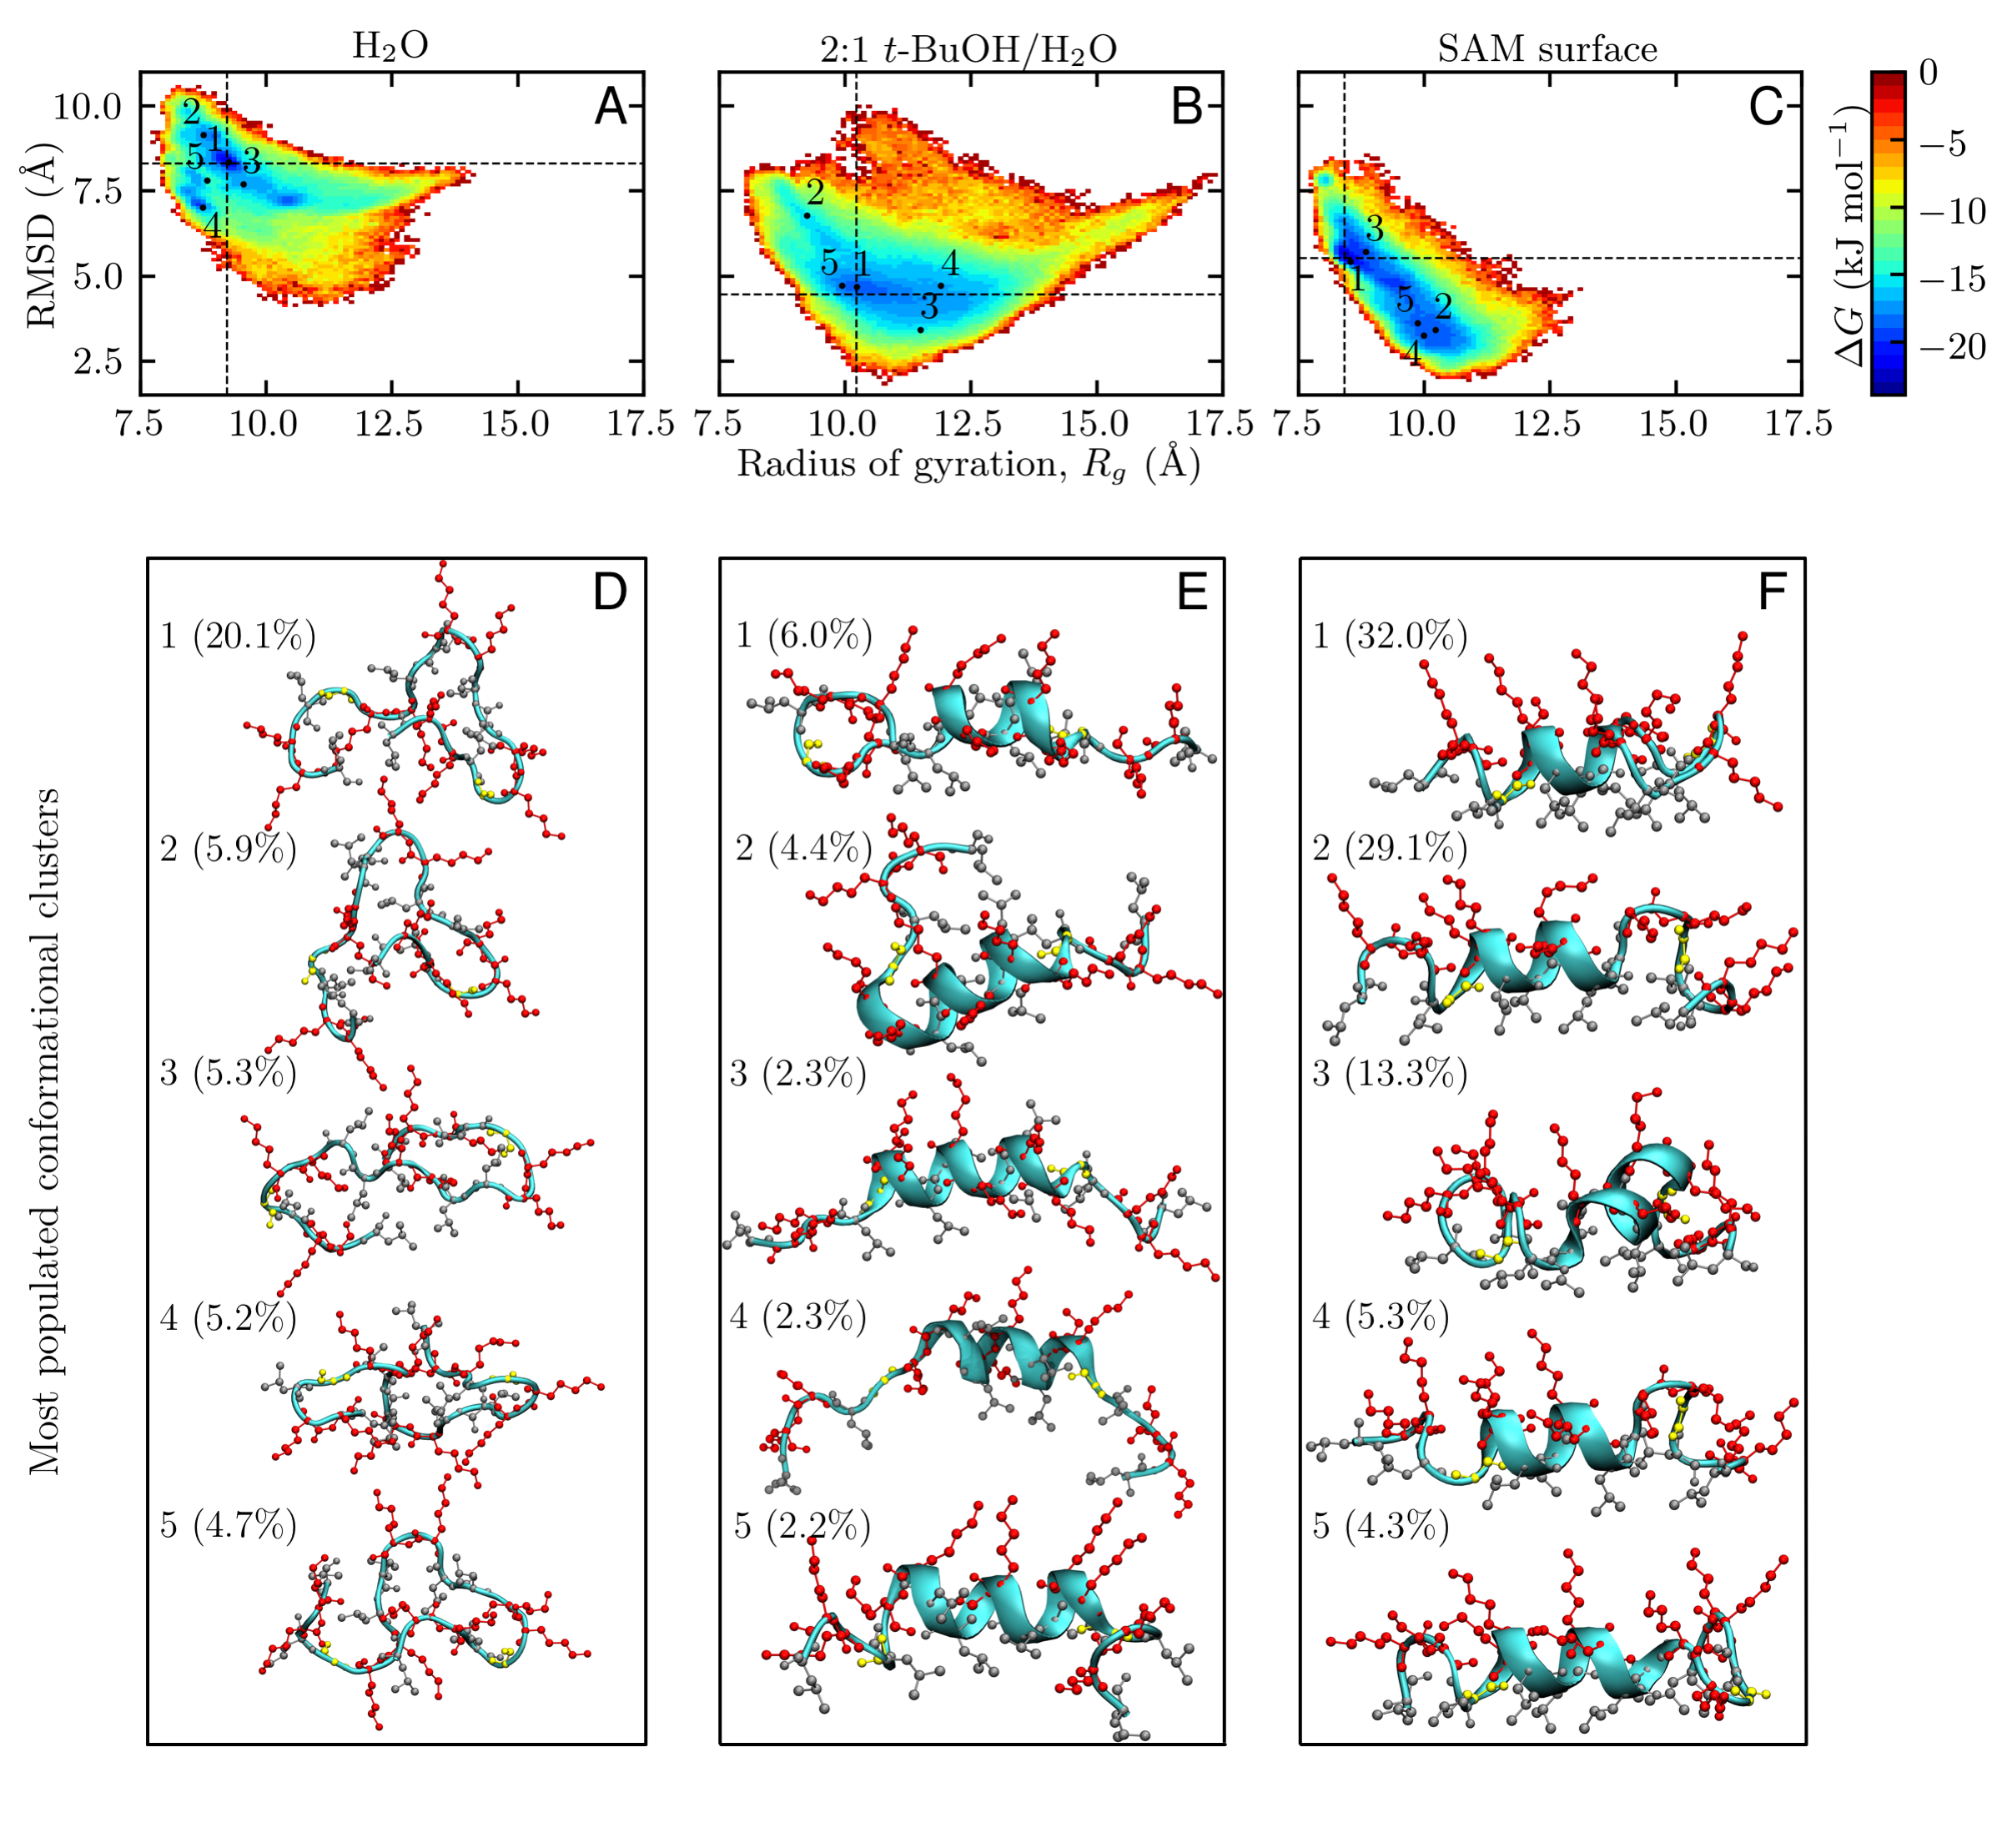
\includegraphics[width=5.50in]{figures-helix/clusters_proofs.png}
    \caption[Free energy surfaces and most populated clusters of \pep{} in each solvent environment]{
        A, B, C: Free energy surfaces of the combined ensemble of structures on \pep{} in the three solvent environments. 
        On the $x$-axis is the radius of gyration of the protein. 
        On the $y$-axis is the backbone RMSD away from a perfectly folded \textalpha{}-helix. 
        The intersection of the dashed lines is the global minimum for each surface. 
        D, E, F: Central structure from each of the top five conformation clusters from the combined ensemble of structures. 
        The central structure was taken from the frame with the lowest RMSD to all the other structures in the cluster. 
        The cyan ribbon represents the protein backbone, the red spheres represent the heavy atoms of the lysine residues, the gray spheres represent the heavy atoms of the leucine residues, and the yellow spheres represent the heavy atoms of the glycine residues. 
        Each structure is labeled with the percentage of the total number of structures that are less than 2.5 \si{\angstrom} backbone RMSD away from the structure shown. 
        A, D: the peptide was dissolved in water. 
        B, E: the peptide was dissolved in \tbawat{}. 
        C, F: the peptide was on the surface of a SAM dissolved in water.
    }
    \label{fig:helix-free_cluster}
\end{figure}

\subsection{Cluster analysis of most populated structures from the simulated ensembles}

To investigate the structures stabilized by the free energy surfaces discussed above, we performed a cluster analysis on the combined ensemble of structures for each of the three solvent environments. 
Because this requires pairwise RMSD calculations, structures were only sampled every 100 ps for this analysis. 
Clusters were identified using the Gromos algorithm\cite{Daura1999} and the gmx cluster module with a cutoff of 2.5 \si{\angstrom} backbone RMSD between clusters in order to visualize common structural motifs throughout the trajectory. 
Figure \ref{fig:helix-free_cluster}D illustrates the central structure of the five most populated conformational clusters of \pep{} in water. 
The central structure of the peptide was taken from the frame with the lowest RMSD from all the other structures in the cluster. 
The label indicates the percentage of the total ensemble of structures that were represented by the cluster. 
In water, all of the most populated clusters were disordered or unfolded conformations, and their $R_g$ and backbone RMSD to an \textalpha{}-helical conformation are labeled on the free energy surface in Figure \ref{fig:helix-free_cluster}A. 
None of the five clusters in water had helical character; 
the hydrophobic leucine residues (gray) were centrally located while the hydrophilic lysine residues (red) were more radially distributed and directed out into the surrounding solution. 
Further, a \textbeta{}-turn motif at the N-terminus, where the peptide turns back on itself and aligns in an anti-parallel fashion, was observed in all five clusters. 
While this motif was too short to be considered a \textbeta{}-strand by the DSSP algorithm and instead was classified as ``bend,'' these residues accounted for the $\sim$0.4 strand character observed in the stacked conformational fractions (Figure \ref{fig:helix-conf_fracs}A and \ref{fig:helix-conf_fracs}B).

Figure \ref{fig:helix-free_cluster}E illustrates the central structure of the five most populated conformational clusters of \pep{} in \tbawat{}, and the corresponding $R_g$ and RMSD of these structures are labeled on the free energy surface in Figure \ref{fig:helix-free_cluster}B. 
All five contained 2-3 helical turns in the middle region of the peptide. 
In contrast to the structures in water, the leucine residues (gray) appeared to be on the opposite side of the helical axis than the hydrophilic lysine residues (red). 
The two terminal regions did not have defined secondary structure. 
They were typically extended, and the residues were classified as ``coil'' by DSSP (Figure \ref{fig:helix-dssp}C and \ref{fig:helix-dssp}D). 
The top five clusters only accounted for 17.2\% of the total ensemble of structures, which implies a large amount of intrinsic disorder for the peptide in \tbawat{} and is consistent with the more diffuse free energy surface (Figure \ref{fig:helix-free_cluster}B. 
Nevertheless, the stacked conformational fractions in Figures \ref{fig:helix-conf_fracs}C,D and the DSSP assignments in Figures \ref{fig:helix-dssp}C,D demonstrate that the majority of the less populated clusters not shown in Figure \ref{fig:helix-free_cluster}E had similar secondary structure in the middle region of the peptide.

Finally, Figure \ref{fig:helix-free_cluster}F illustrates the central structure of the five most populated conformational clusters of \pep{} on the surface of the SAM, and the corresponding $R_g$ and RMSD of these structures are labeled on the free energy surface in Figure \ref{fig:helix-free_cluster}C. 
Again, all five of the clusters displayed 2-3 helical turns in the middle region of the peptide, and the leucine (gray) and lysine (red) residues were clearly separated from each other. 
For reference, these structures were oriented such that the SAM surface (not shown) was below the peptide, adjacent to the leucine residues. 
In contrast to the peptide in \tbawat{}, the terminal regions of the peptide at the SAM surface had high curvature. 
The residues in this region were classified as ``turn'' by the DSSP algorithm because they lacked the repeating hydrogen bonds to be classified as helical (Figures \ref{fig:helix-dssp}E,F). 
Furthermore, the five clusters shown in Figure \ref{fig:helix-free_cluster}F accounted for 84.0\% of the total ensemble of structures, which implies that the peptide on the surface was significantly more structured than in either of the two solutions.

A comparison of the coverage of the total ensemble of structures against the number of clusters is shown in Figure \ref{fig:helix-coverage}. 
The ensemble of structures of \pep{} on the SAM was covered by significantly fewer clusters than \pep{} in either solution, consistent with the distinct minima of $\Delta G$ apparent on the free energy surface. 
In turn, the ensemble of structures of \pep{} in \ce{H2O} was covered by fewer clusters than \pep{} in \tbawat{}. 
This is again consistent with the distinct minima with slightly higher $\Delta G$ apparent on the free energy surface of \pep{} in \ce{H2O} and with the diffuse free energy surface with the highest minimum $\Delta G$ for \pep{} in \tbawat{}. 
This implies that the structural regularity of \pep{} increased from \tbawat{}, to \ce{H2O}, to the SAM surface, revealing a particular advantage of complementing the experimental studies with MD simulations. 
Only the average structure may be observed in the bulk experimental CD spectra but the simulations reveal a dynamic distribution of structures that all contribute to the overall experiment. 

\begin{figure}
    \center
    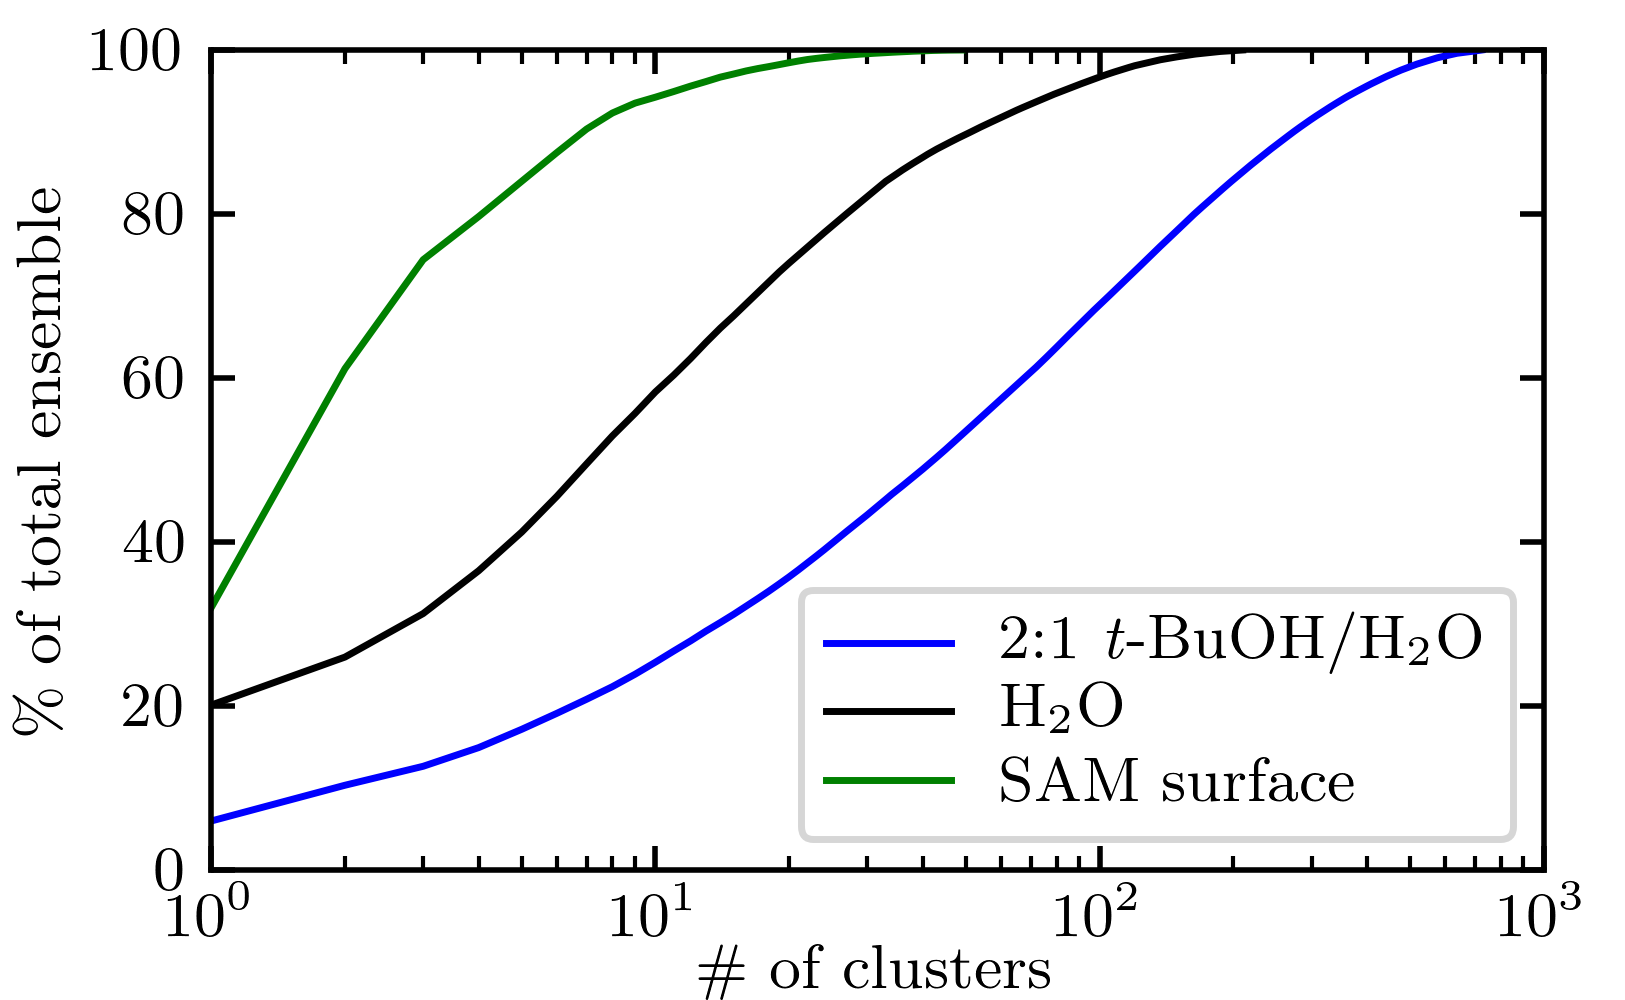
\includegraphics[width=\single]{figures-helix/clust-size.png}
    \caption[Ensemble converage by conformational clusters]{
        The percentage of coverage of the total ensemble of structures against the number of clusters for the peptide in water (black), in \tbawat{} (blue), and on the surface of a SAM (green).
    }
    \label{fig:helix-coverage}
\end{figure}

\subsection{Conformational fractions are consistent with experimental CD spectra}

While the central structures in Figure \ref{fig:helix-free_cluster} are consistent with our expectations from the experimental CD spectra in Figure \ref{fig:helix-cd_spectra}, it is not clear if the structural differences observed are enough to account for the change in the spectra. 
This is further complicated by the fact that conformations with large amounts of disorder, such as those of \pep{} in these three systems, do not always result in well-defined secondary structures that are apparent from CD spectroscopy. 
More advanced techniques, such as chiral sum frequency generation, can more quantitively determine the degree of each secondary structure exhibited by the peptide on surfaces\cite{Fu2011}. 
However, because of the wide spread use of CD as a measurement of secondary structure, we: 
1) compared the secondary structure calculated from the experimental spectra to the secondary structures from simulation; 
and 2) compared calculated CD spectra from the MD trajectories to the experimental CD spectra. 
Although these comparisons have the same goal, each relies on different spectral analysis tools, and are thus two orthogonal ways to compare the experimental CD data to the calculated MD structures. 
In order to accomplish the first comparison strategy, we deconvoluted the experimental spectra into conformational fractions using the online deconvolution server BeStSel\cite{Micsonai2015, Micsonai2018}. 
This routine uses a basis set of CD spectra of proteins with known structure to estimate the fraction of secondary structures that would reconstitute the given CD spectrum. 
The spectra of the peptide in water and in \tbawat{} were input as is from Figure \ref{fig:helix-cd_spectra}, and good fits, with normalized RMSDs (NRMSDs) of less than 0.02, were obtained. 
However, for the spectrum of the peptide on the SAM surface (green spectrum in Figure \ref{fig:helix-cd_spectra}), we did not obtain an acceptable fit with the experimental data.
There were three reasons for this failure. 
First, the baseline of the spectrum was not consistent with the two spectra collected in solution. 
This created a significant amount of error since all of the BeStSel basis spectra have zero ellipticity at 250 nm. 
Second, the concentration of the peptide on the surface was not consistent with the other two experiments. 
The fits are highly dependent on accurate concentration estimates, since weak signals can occur from either poorly organized secondary structures or low concentrations of peptide. 
Third, the spectrum was red-shifted by 1 nm compared to the solution-phase spectra, probably due to the presence of the hydrophobic surface \cite{Chen1997}. 
The red-shift moved the characteristic transitions of \textalpha{}-helices to 209 and 223 nm, which caused the BeStSel algorithm to underestimate the amount of helical character. 
We therefore modified the experimental CD spectrum of \pep{} on the SAM surface in three ways: 
1) we corrected the baseline by forcing it to zero at 250 nm; 
2) we scaled the spectrum by a factor of 10 to account for the reduced concentration of the peptide on the surface compared to solution; and 
3) we blue-shifted the spectrum by 1 nm to place the absorption minima at 208 nm and 222 nm. 
A good fit for this corrected spectrum was obtained with NRMSD of less than 0.02. 

The average conformational fractions from the simulations (excluding the equilibration times discussed above) and the conformational fractions determined by BeStSel are shown in Table \ref{tbl:helix-frac_bestsel}. 
Fractions that differ by less than 0.05 are shown in bold. 
For \pep{} in water, the conformational fraction in simulation and from the BeStSel deconvolution were in strong agreement for the fraction of the peptide that was either in a helical (0.001 and 0.017, for simulation conformational fraction and BeStSel estimation respectively) or an unfolded structure (0.527 and 0.550). 
However, the MD trajectories underestimated the fraction of turn character (0.042 and 0.188) and overestimated the fraction of strand character (0.430 and 0.245). 
This is consistent with investigations that demonstrated that OPLS can be biased toward extended and \textbeta{}-turn conformations\cite{Best2011, Smith2015}. 
For \pep{} in \tbawat{}, the conformational fractions were in good agreement for all four categories: helical (0.276 and 0.261), turn (0.130 and 0.150), strand (0.173 and 0.184), and unfolded (0.421 and 0.405). 
Finally, for \pep{} on the surface of the SAM, the conformational fractions in simulation and from the BeStSel deconvolution were in good agreement for the helical (0.318 and 0.278) and unfolded fractions (0.223 and 0.221). 
However, the simulations yielded a slightly higher turn fraction (0.296 and 0.197) and a slightly lower strand fraction (0.163 and 0.304) than the BeStSel estimates. 
There are two possible sources for this disagreement for the peptide at the SAM: 
1) there is a large amount of noise in the experimental data of the peak at 200 nm, which is due to the difficulty of taking such spectra on a surface; and 
2) there is greater error in estimating the concentration of the peptide on a surface than in solution. 
The accuracy of the BeStSel deconvolution is heavily dependent on both of these factors. 
A third possible source of this discrepancy could be again the choice of force field used in the simulations, as it has been suggested qualitatively that OPLS-AA may over represent random coil character on SAM surfaces\cite{Collier2012}. 
Since the onset of the present work, a new force field (CHARMM36m) has been shown to be accurate for intrinsically disordered peptides\cite{Huang2017}, which might ameliorate the discrepancies in Table \ref{tbl:helix-frac_bestsel}. 
We are investigating this in ongoing simulations using the CHARMM36m force field. 
Nevertheless, the agreement between the fractions from the deconvolution and the simulations is striking and gives us confidence in the accuracy of the simulations.

\begin{table}
    \caption[Conformational fractions from simulation and conformational fractions from CD spectra]{Average conformational fraction from simulation and conformational fractions from BeStSel\cite{Micsonai2015, Micsonai2018} CD spectra deconvolution.}
    \begin{center}
        \resizebox{\double}{!}{
    \begin{tabular}{c|cccc|cccc}
    \toprule
        Solvent        & \multicolumn{4}{c}{Calculated} & \multicolumn{4}{c}{BeStSel deconvolution from experiment} \\
        & Helix & Turn & Strand & Unfolded & Helix & Turn & \textbeta{}-sheet & Others \\
    \midrule
        \ce{H2O} & \textbf{0.001} & 0.042 & 0.430 & \textbf{0.527} & \textbf{0.017} & 0.188 & 0.245 & \textbf{0.550} \\
        2:1 \ce{H2O}:\emph{t}-BuOH & \textbf{0.276} & \textbf{0.130} & \textbf{0.173} & \textbf{0.421} & \textbf{0.261} & \textbf{0.150} & \textbf{0.184} & \textbf{0.405} \\
        SAM surface   & \textbf{0.318} & 0.296 & 0.163 & \textbf{0.223} & \textbf{0.278}* & 0.197* & 0.304* & \textbf{0.221}* \\
    \bottomrule
    \end{tabular}
}
    \end{center}
    \textbf{Bold} indicates that the calculated fraction is within $\pm 0.05$ of the BeStSel estimated counterpart. 
    *BeStSel deconvolution was performed on the CD spectrum of \pep{} on the SAM after applying a baseline correction, a 1 nm red-shift, and a scale-factor of 10. 
    See main text for details.
    \label{tbl:helix-frac_bestsel}
\end{table}

While the secondary structure estimated from the experimental spectra agreed with the simulations, we also calculated CD spectra from the MD trajectories in order to compare to experimental spectra (the second strategy described above). 
In order to accomplish this, we calculated the CD line spectrum for structures extracted every 100 ps in each of the six simulations using the DichroCalc portal \cite{Bulheller2009, Jasim2018}. 
Each line spectrum was convoluted with a Gaussian band shape using an in-house Python code to produce a continuous CD spectrum. 
We explored a range of bandwidths from 9 nm to 14 nm, but found that this did not change the observations and conclusions reported below (data not shown). 
Here, we show the spectra calculated with a bandwidth of 10 nm. 
The spectra were averaged across 125 ns time windows and are shown in Figure \ref{fig:helix-calc_cd}. 
For each simulation that started from a folded conformation (Figures \ref{fig:helix-calc_cd}A,C,E), the first 125 ns averaged CD spectrum (dark blue trace) had a distinct minimum around 208 nm and 222 nm, a distinctive characteristic of the CD spectra of \textalpha{}-helices\cite{Holzwarth1965, Woody1967, Johnson1988, Berova2000circular, Kelly2005}.
For the simulation in water starting from a folded state (Figure \ref{fig:helix-calc_cd}A), these two minima disappeared as the peptide unfolded in solution, and then a positive peak appeared around 200 nm (green to yellow traces). 
This transition is associated with anti-parallel \textbeta{}-sheets\cite{Greenfield1969, Manning1988} and coincided with the appearance of strand character in the stacked conformational fraction (Figure \ref{fig:helix-conf_fracs}A). 
For the simulation in water starting from an unfolded state (Figure \ref{fig:helix-calc_cd}B), the two minima at 208 nm and 222 nm were present only weakly in the first few averaged spectra, when the peptide sampled some weakly helical configurations (Figure \ref{fig:helix-calc_cd}B). 
These two minima then disappeared and a positive peak at 200 nm appeared for the remainder of the trajectory. 
For the simulation in \tbawat{} starting from the folded state (Figure \ref{fig:helix-calc_cd}C), the two minima associated with \textalpha{}-helices (208, 222 nm) were present for each averaged window. 
The spectra were relatively consistent in each window with only minor changes in the intensity of the peaks. 
For the simulation in \tbawat{} starting from the unfolded state (Figure \ref{fig:helix-calc_cd}D), the first window averaged spectrum (0-125 ns, dark blue trace) had a positive peak around 200 nm. 
The positive peak disappeared in subsequent windows, replaced by two weak negative peaks around 208 nm and 222 nm. 
These two negative peaks grew in intensity until 1 \textmu{}s. 
The peptide then sampled some unfolded configurations (Figure \ref{fig:helix-conf_fracs}D), resulting in a final window averaged spectrum that had very weak minima at 208 and 222 nm (Figure \ref{fig:helix-calc_cd}D, yellow trace). 
Nevertheless, the majority of the spectra for the simulation of \pep{} in \tbawat{} had minima at 208 nm and 222 nm. 
For the simulation on the surface of the SAM starting from the folded state (Figure \ref{fig:helix-calc_cd}E), the window averaged CD spectra all had characteristic minima at 208 and 222 nm, with stronger intensity than that of the peptide in \tbawat{}, indicating more helical character. 
For the simulation on the surface of the SAM starting from the unfolded state (Figure \ref{fig:helix-calc_cd}F), all window averaged CD spectra had the same minima. 
The spectrum for 0-125 ns (dark blue trace) had the weakest minimum, since the peptide in this window was still folding. 
In subsequent windows, the strength of the minima tended to increase, again greater than the spectra of \pep{} in \tbawat{}.

\begin{figure}
    \center
    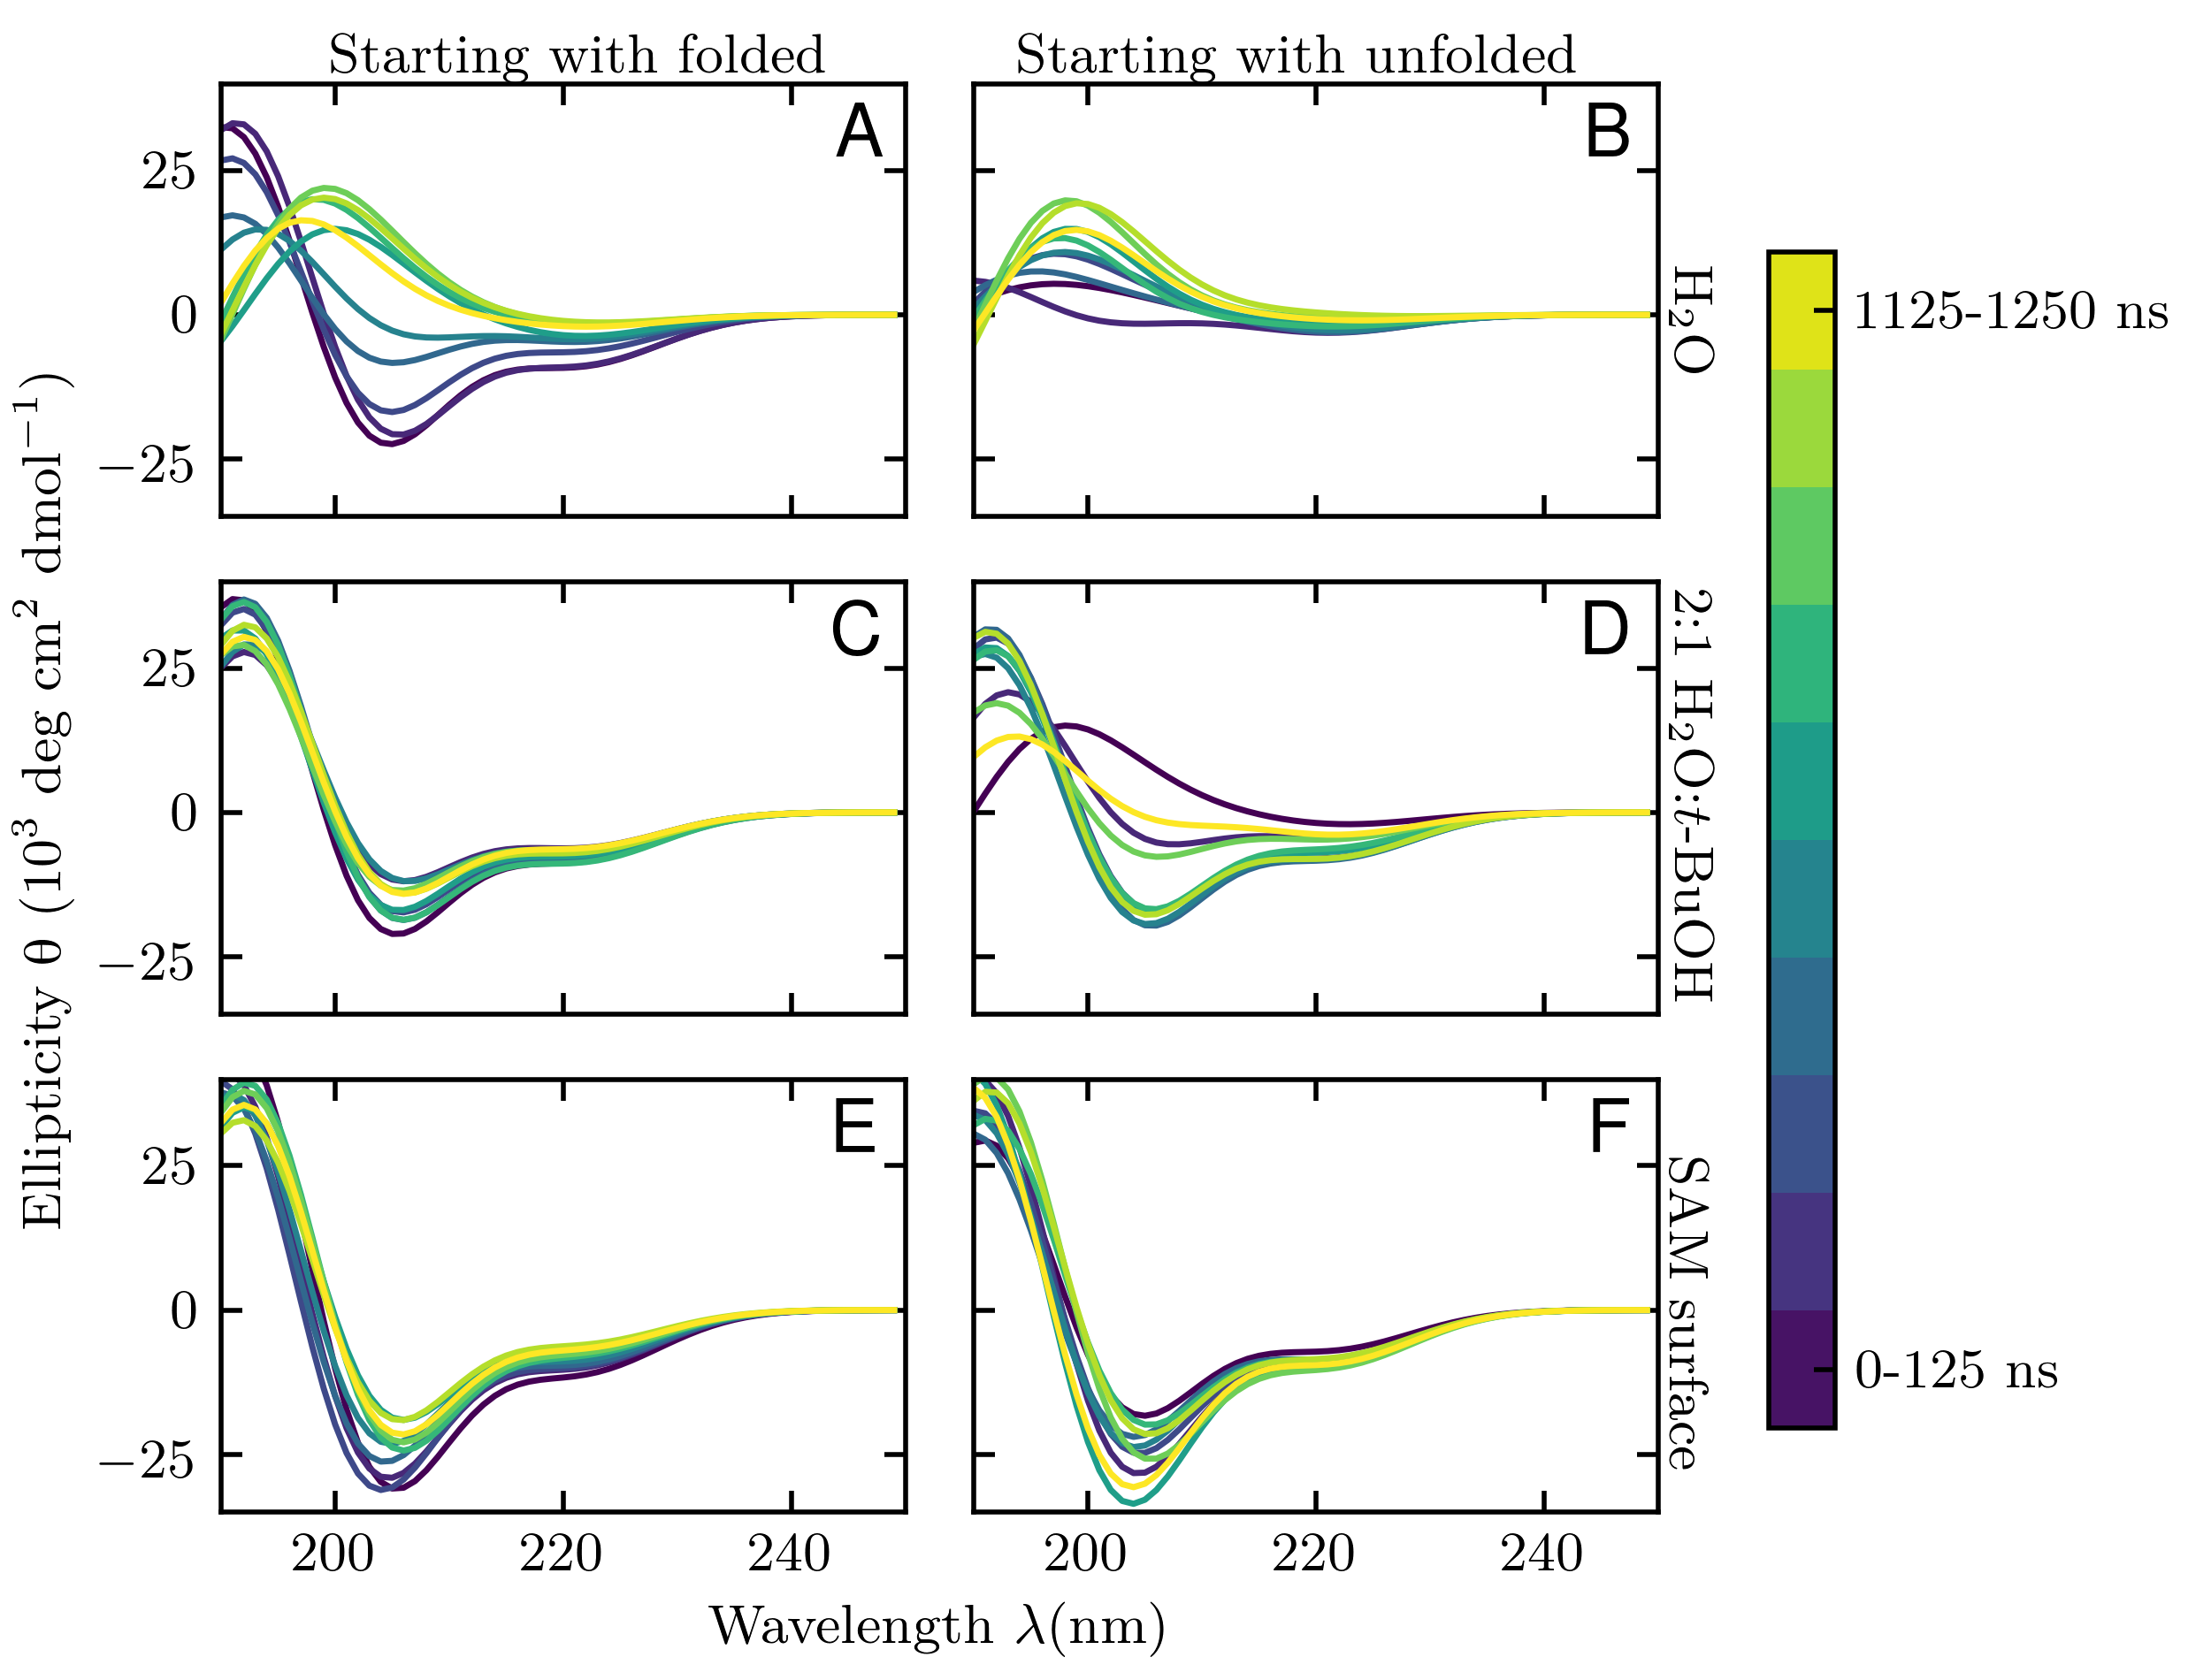
\includegraphics[width=\double]{figures-helix/cd_spectra_hirst_time_resolved.png}
    \caption[Computed CD spectra of \pep{} in three solvent environments]{
        Computed CD spectra calculated from the MD trajectories using the DichroCalc portal and the Hirst basis set \cite{Hirst1998, Besley1999}.
        Each spectrum was convoluted with a Gaussian function with bandwidth of 10 nm. 
        Spectra were calculated every 100 ps, and each line represents a 125 ns average and is colored by its time. 
        A, C, E: \pep{} began the simulation in an \textalpha{}-helical conformation. 
        B, D, F: \pep{} began the simulation unfolded. 
        A, B: the peptide was dissolved in water. 
        C, D: the peptide was dissolved in \tbawat{}. 
        E, F: the peptide was on the surface of a SAM dissolved in water.
    }
    \label{fig:helix-calc_cd}
\end{figure}

The total averaged spectrum from the entire ensemble of structures in each solvent (excluding the equilibration times discussed above) are shown in Figure \ref{fig:helix-avg_cd}A. 
For the averaged spectrum of \pep{} in water (Figure \ref{fig:helix-avg_cd}A, black), there was a positive peak around 200 nm, and a very weak minimum at 222 nm. 
The positive peak was a result of the strand character and was not consistent with the experimental spectrum (Figure \ref{fig:helix-cd_spectra}, black). 
While this may be a result of our simulations slightly overestimating the strand character of \pep{} in water, the CD spectra of \textbeta{}-sheets are extremely sensitive to the exact configuration of the structure, and minor differences in the alignment of the \textbeta{}-sheet can result in large differences in the observed spectrum \cite{Micsonai2015}.
The difference in the computed spectrum and the experimental spectrum, therefore, may be due only to minor differences in the tilt of the \textbeta{}-sheet. 
However, both the computed and experimental spectra indicated no helical character, which was borne out in the simulations. 
For the computed spectrum of \pep{} in \tbawat{} (Figure \ref{fig:helix-avg_cd}A, blue), there were distinct negative transitions at 208 and 222 nm indicative of helical character. 
The computed spectrum was in good qualitative agreement with the experimental spectrum (Figure \ref{fig:helix-cd_spectra}, blue). 
Finally, the computed spectrum \pep{} on the surface of the SAM (Figure \ref{fig:helix-avg_cd}A, green) contained these same two negative peaks with greater intensity. 
While the absolute intensities in the experimental spectra cannot be compared to each other because of the difficulty in determining the concentration on the surface, the resolution of the two peaks in the experimental spectrum implied stronger helical character (Figure \ref{fig:helix-cd_spectra}, green). 
This was indeed captured by the computed spectrum. 
The relative intensity between the two peaks, however, was not captured, which could be due to the choice of the Hirst basis set\cite{Hirst1998, Besley1999} for the calculation. 
CD spectra computed using the Woody basis set\cite{Woody1999} shown in Figure \ref{fig:helix-avg_cd}B qualitatively matched the experimental spectrum for \pep{} on the SAM surface. 
However, the spectra calculated using this basis set failed to capture the relative intensity of the two peaks for \pep{} in \tbawat{}. 
Taken together, however, the calculated CD spectra were in qualitative agreement with the experimental spectra, which, when combined with the quantitative agreement of the conformational fractions from simulation and the BeStSel deconvolution, gives us confidence that we can accurately simulate the peptide in these complex environments.

\begin{figure}
    \center
    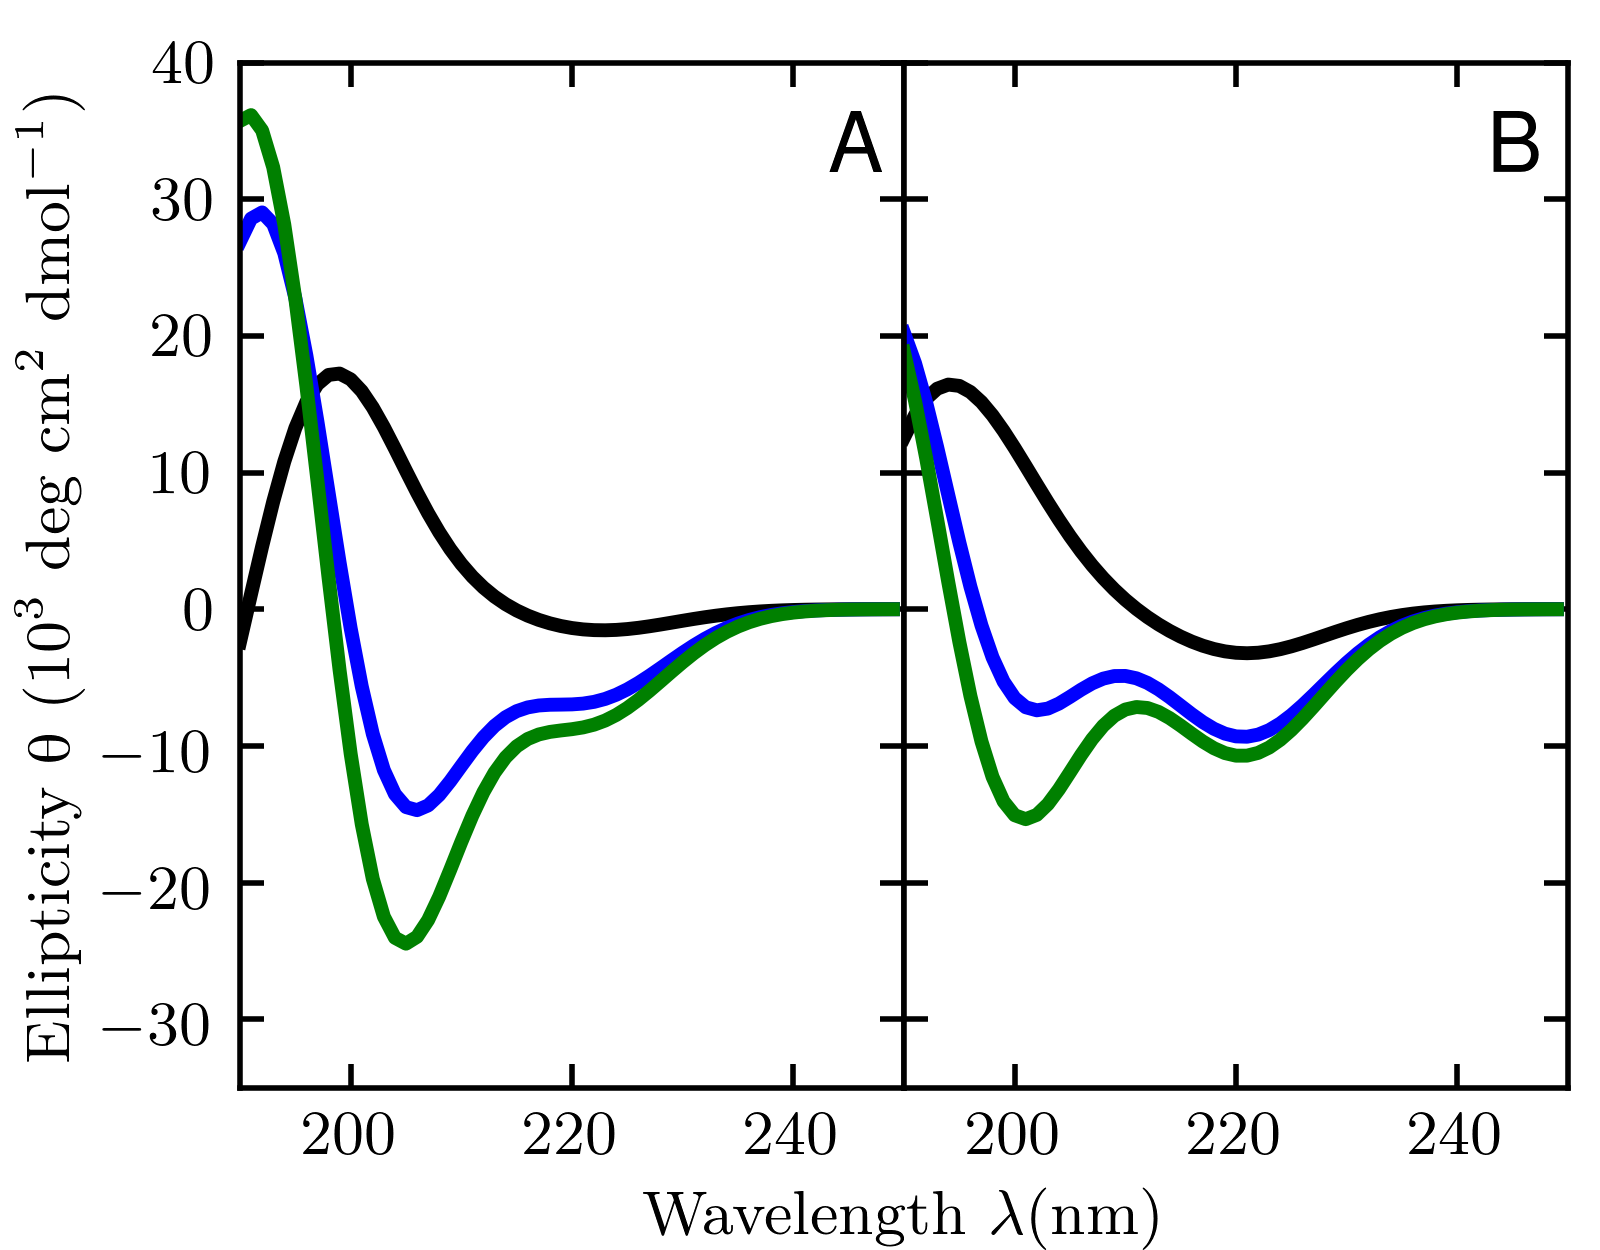
\includegraphics[width=\single]{figures-helix/combined_cd_spectra.png}
    \caption[Average computed CD spectra of \pep{}]{
        Ensemble averaged CD spectra computed from MD simulations of \pep{} in water (black), \tbawat{} (blue), and on the surface of a SAM (green). 
        Spectra were computed using the DichroCalc web portal and either the Hirst basis set\cite{Hirst1998, Besley1999} (A) or the Woody basis set\cite{Woody1999} (B).
    }
    \label{fig:helix-avg_cd}
\end{figure}

%%%%%%%%%%%%%%%%%%%%%%%%%%%%%%%%%%%%%%%%%%%%%%%%%%%%%%%%%%%%%%%%
%%%%%%%%%%%%%%%%%%%%%%%%%%%%%%%%%%%%%%%%%%%%%%%%%%%%%%%%%%%%%%%%
\section{Discussion}\index{helix-discussion}
%%%%%%%%%%%%%%%%%%%%%%%%%%%%%%%%%%%%%%%%%%%%%%%%%%%%%%%%%%%%%%%%
%%%%%%%%%%%%%%%%%%%%%%%%%%%%%%%%%%%%%%%%%%%%%%%%%%%%%%%%%%%%%%%%

Our results demonstrate that the widely available OPLS-AA force field can accurately model our charged peptide \pep{} in these two complex environments: 
1) in a binary solvent (\tbawat{}); and 
2) on a SAM surface. 
The agreement between simulations that started at different conformations (folded and unfolded) showed that our results are not heavily influenced by our starting structure. 
The accuracy of these structures was demonstrated by: 
1) the quantitative agreement between the simulated conformational fractions and the fractions estimated by BeStSel deconvolution (Table \ref{tbl:helix-frac_bestsel}); and 
2) the qualitative agreement between the spectra computed from MD trajectories using DichroCalc (Figure \ref{fig:helix-avg_cd}) and the experimental spectra (Figure \ref{fig:helix-cd_spectra}). 
In particular, conformational transitions between helical and \textbeta{}-sheet structures have profound implications on amyloid plaque diseases such as Alzheimer's, Parkinson's, and Huntington's diseases\cite{Jahn2006, Chiti2009, Abedini2009, Hoop2016, Kim2016, Mondal2019}, particularly when the conformational change is induced by an interface \cite{Chi2010, Moores2011, Ho2018}. 
Here, we have shown that \pep{} switches between a \textbeta{}-turn motif in water, a partially folded helix in \tbawat{}, and a folded helix on a hydrophobic surface, demonstrating the utility of this model peptide for research into the molecular mechanisms of such diseases. 
Accurate simulations are paramount to this effort. 
Further, the conformational changes observed in simulation can guide experimental strategies to incorporate biomolecules on surfaces and provide foundational knowledge on the stability of protein structures in such environments.

Because of the unique sequence of our peptide that was designed to fold at a polar/apolar interface, the results presented here should not be used to assume that OPLS will be able to accurately model all conformational changes on a surface. 
The accuracy of any force field on a peptide in such an environment must be validated against experimental data. 
Nevertheless, the accuracy demonstrated here allows us to test specific mechanistic questions about how this peptide interacts with different surface environments. 
For example, in order to keep the peptide near the surface during the equilibration and heating processes, harmonic restraints were added to hold the glycine residues to the appropriate distance from the SAM. 
For the simulations discussed above, these restraints were removed for the production phase simulations, so that the peptide was unrestrained on the surface. 
However, in the experiment to which we are comparing our results, the peptide is covalently bound to the SAM through a triazole linker (Figure \ref{fig:helix-linker}). 
We do not have any experimental evidence to determine whether the peptide folds before reacting with the SAM layer, or if the peptide reacts and then folds. 
Further, the SAMs in these simulations were nearly perfectly ordered but by relaxing this, the effect of the order of the SAM on the peptide structure can now be tested \emph{in silico}. 
Below, we introduce two additional sets of simulations that test these experimental questions: 
1) the influence of the number of binding sites holding the peptide near the SAM surface on the folding process; and 
2) the effect of structural order of the SAM on the equilibrium structure of the peptide. 
Using these two additional sets of simulations, we identify two hypotheses regarding the mechanistic details of the peptide folding on the surface that can be specifically tested by further experiments. 

In order to test the effect of the number of binding sites holding the peptide to the SAM surface, we ran four additional 1.25 \textmu{}s simulations where one or both of the harmonic restraints that bind the glycine residues to the SAM (see Section \ref{helix-anneal}) were kept for the production phase, instead of removing them as in the simulations reported above. 
The stacked conformational fractions for these additional simulations are shown in Figure \ref{fig:helix-bounds}, and the quantitative results (not including values before the 150 ns equilibration time) are shown in Table \ref{tbl:helix-bounds}. 
With both glycine residues bound, starting from a folded state (Figure \ref{fig:helix-bounds}A), the peptide remained folded through the entire simulation with average conformational fractions consistent with the unrestrained simulations shown in Table \ref{tbl:helix-frac_bestsel} (helix: 0.272, turn: 0.290, strand: 0.205, and unfolded: 0.233). 
However, starting from an unfolded conformation (Figure \ref{fig:helix-bounds}B), the peptide did not fold to the same extent, resulting in very different conformational fractions (helix: 0.083, turn: 0.083, strand: 0.350, and unfolded: 0.484). 
In contrast, with only one glycine bound (Figures \ref{fig:helix-bounds}C,D), the peptide reached similar conformational fractions from the folded state (helix: 0.278, turn: 0.264, strand: 0.179, and unfolded: 0.280) as from the unfolded state (helix: 0.275, turn: 0.315, strand: 0.162, and unfolded: 0.248). 
In both of these simulations, the average conformational fraction was consistent with the conformational fractions of the simulations with no restraints (Table \ref{tbl:helix-frac_bestsel}). 
Indeed, in every simulation of \pep{} on the SAM surface, the average conformational fractions were consistent \emph{except} when the peptide was unfolded and restrained at both glycine residues. 
These results imply that the two restraints prevented the peptide from folding. 
This in turn suggests the hypothesis that the peptide must be folded before the second covalent attachment occurs. 
We are currently testing this hypothesis experimentally. 

\begin{figure}
    \center
    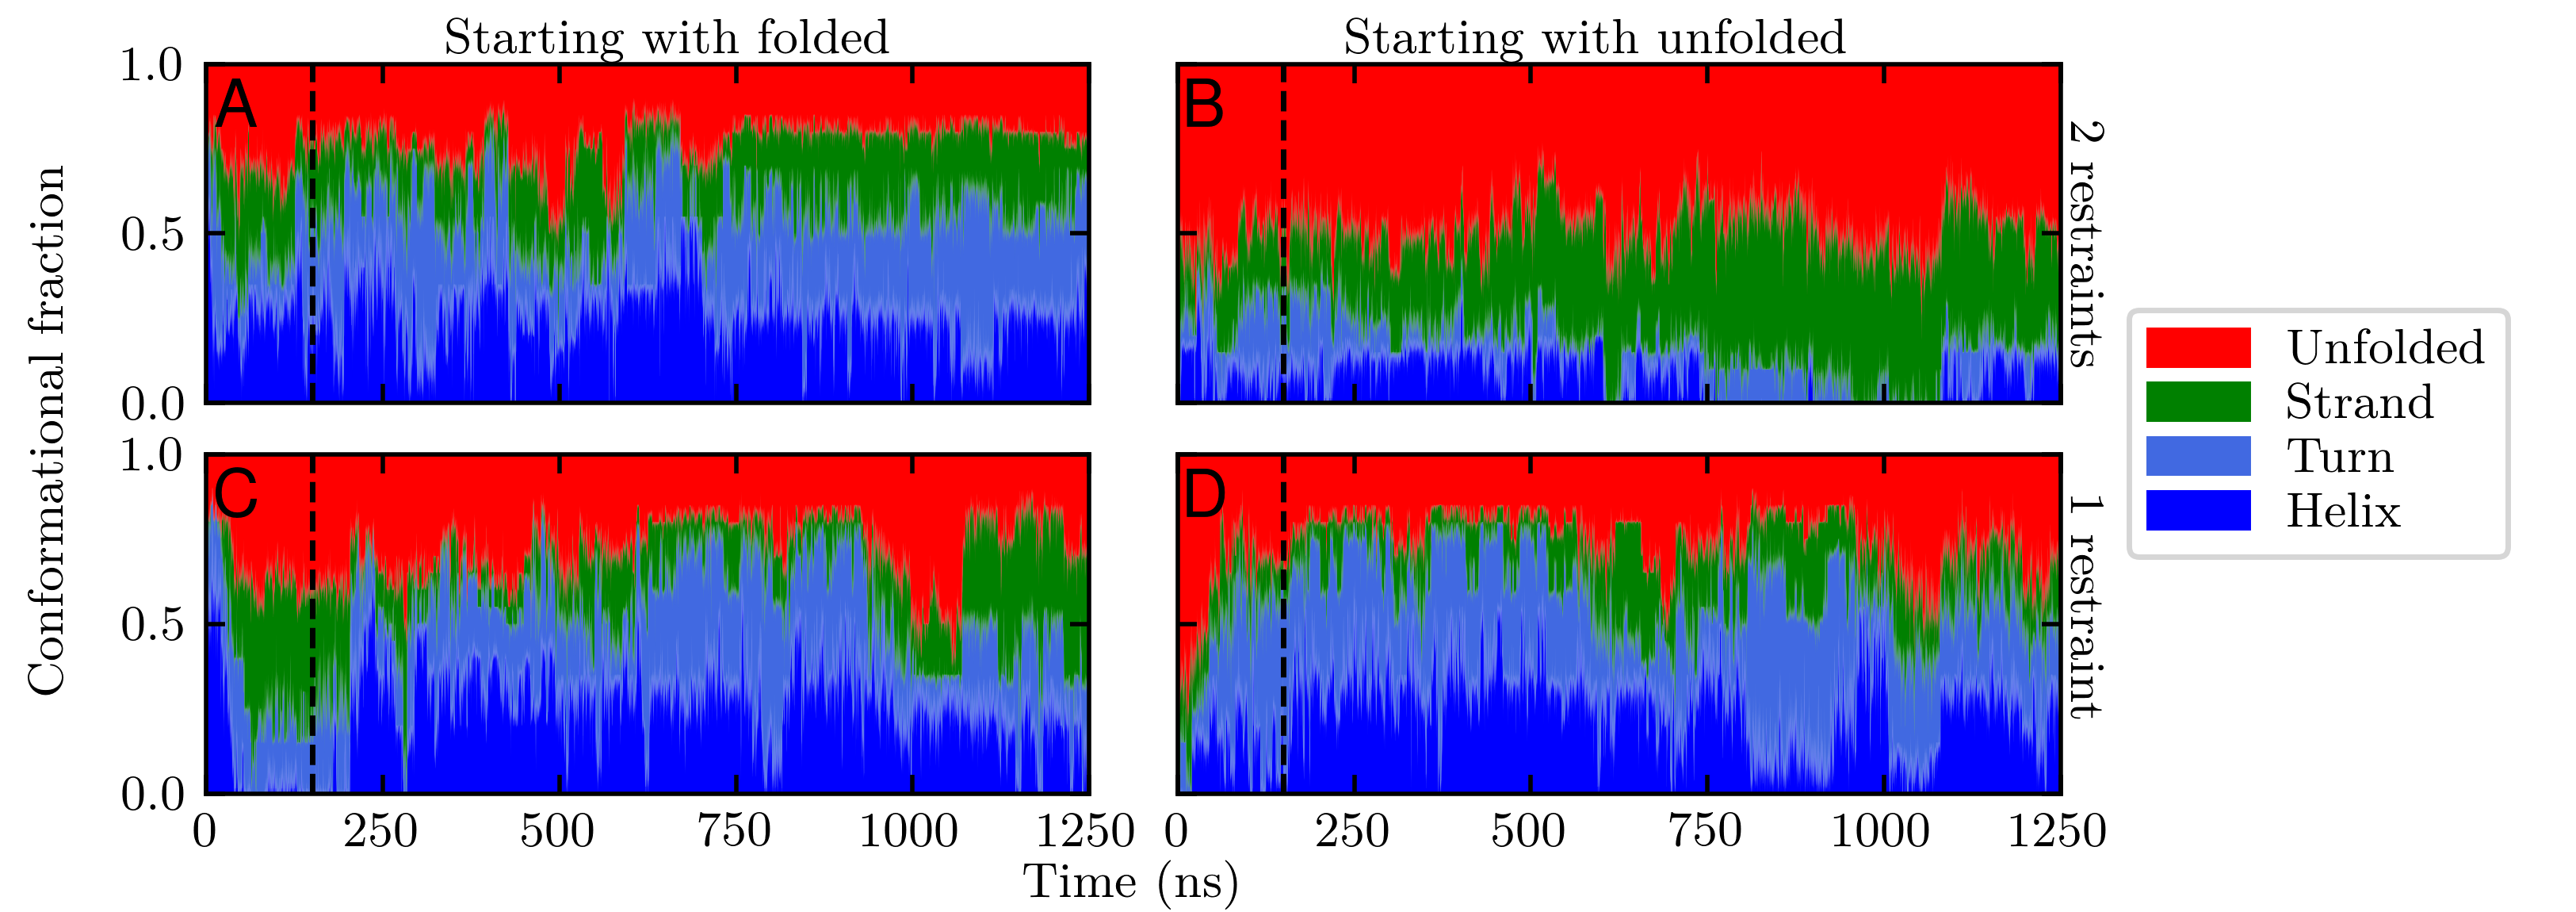
\includegraphics[width=\double]{figures-helix/bounds_helicity.png}
    \caption[Stacked conformational fractions of \pep{} with one or both glycines bound]{
        Stacked conformational fractions of \pep{} on the surface of SAM from additional simulations in which either one or both glycine residues were harmonically restrained to the SAM. 
        A, C: \pep{} began the simulation in an \textalpha{}-helical conformation. 
        B, D: \pep{} began the simulation unfolded. 
        A, B: \pep{} was harmonically restrained to the SAM at both glycine residues. 
        C, D: \pep{} was harmonically restrained to the SAM at only one of the glycine residues. 
        The black dashed lines represent the equilibration time. 
        The data after this mark was averaged and is presented in Table \ref{tbl:helix-bounds}.
    }
    \label{fig:helix-bounds}
\end{figure}

\begin{table}
    \caption[Conformational fractions of \pep{} with one or both glycines bound]{Average conformational fractions from simulations of \pep{} on the surface of a SAM in which either one or both of the glycine residues in the peptide are harmonically restrained to the SAM.}
    \begin{center}
     \resizebox{\double}{!}{
     \begin{tabular}{c|cccc|cccc}
    \toprule
    Number of  & \multicolumn{4}{c}{From folded} & \multicolumn{4}{c}{From unfolded} \\
    harmonic restraints & Helix & Turn & Strand & Unfolded & Helix & Turn & Strand & Unfolded \\
    \midrule
    2 & 0.272 & 0.290 & 0.205 & 0.233 & 0.083 & 0.083 & 0.350 & 0.484 \\
    1 & 0.278 & 0.264 & 0.179 & 0.280 & 0.275 & 0.315 & 0.162 & 0.248 \\
    \bottomrule
    \end{tabular}
    }
    \end{center}
    \label{tbl:helix-bounds}
\end{table}

In order to investigate the effect of greater structural disorder within the SAM on the equilibrium structure of the surface-bound peptide, we loosened the harmonic restraints on the decanethiol molecules to $10^3$ kJ mol$^{-1}$ nm$^{-2}$ during the annealing stage of the system preparation (as opposed to $10^7$ kJ mol$^{-1}$ nm$^{-2}$ used for the preparation of the simulations above). 
This allowed molecules within the SAM to shift during the annealing process and resulted in a slightly more disordered SAM surface. 
An illustration of the ``ordered'' and ``disordered'' SAMs are shown in Figure \ref{fig:helix-disordered_sam}A and \ref{fig:helix-disordered_sam}B along with a density profile of the two surfaces in Figure \ref{fig:helix-disordered_sam}C. 
For the ordered SAM, sharp peaks in the density profile indicate the repetitive pattern of the sulfur and each carbon atom in the decanethiol over the entire SAM structure. 
When the restraints were loosened, the atoms of the SAM shifted during the annealing stages, resulting in a less well defined density profile, and indicating a more disordered SAM. 
In order to determine the effect of this disordered structure on the resulting fold of the surface-bound peptide, the simulations using this disordered SAM were run with harmonic restraints between the SAM and both, one, or none of the peptide's glycine residues for 1.25 \textmu{}s each. 
The stacked conformational fractions of these trajectories using a disordered SAM are shown in Figure \ref{fig:helix-disorder}. 
The averaged conformational fractions (not including the fractions before the equilibration time) are shown in Table \ref{tbl:helix-disorder}. 
Starting from a folded conformation and restrained to the SAM at both glycine residues (Figure \ref{fig:helix-disorder}A), the peptide remained folded for the entire trajectory, resulting in high helical content and conformational fractions consistent with the previous simulations on the ordered SAM surface (helix: 0.322; turn: 0.218; strand: 0.159; and unfolded: 0.302). 
However, starting from the unfolded state with two restraints (Figure \ref{fig:helix-disorder}B), the peptide did not fold and displayed low helicity (helix: 0.052; turn: 0.156; strand: 0.291; and unfolded: 0.501). 
The lack of agreement between these two simulations from simulation times that produced consistent results with unrestrained peptide reinforces our previous hypothesis; the second covalent attachment adds a large energy barrier between the folded and unfolded states that prevents the peptide from folding (or unfolding) on the SAM surface, and that \pep{} likely folds before the second bond to the SAM is formed.

\begin{figure}
    \center
    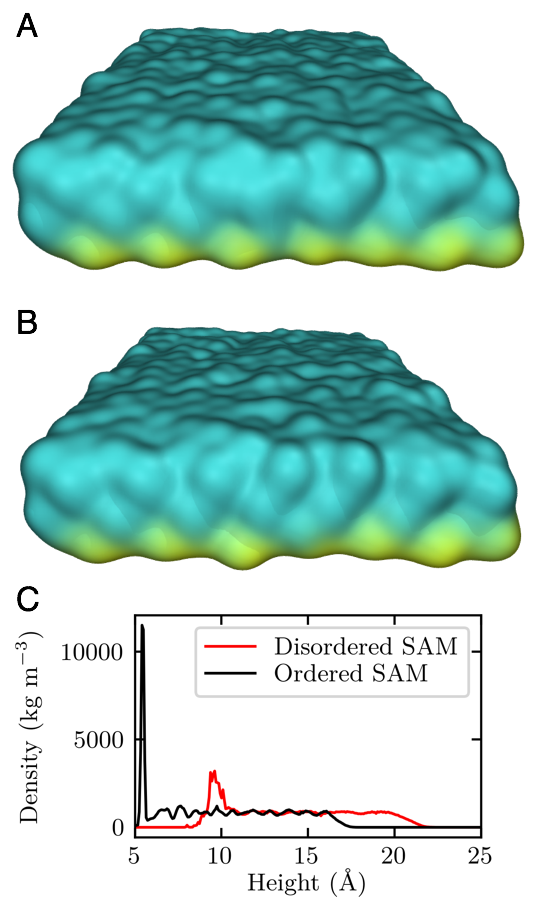
\includegraphics[width=\single]{figures-helix/order_figures.png}
    \caption[Comparison of the ordered and disordered SAM]{
        Surface filling representations of the more ordered SAM (A) used for the simulations with data presented in Figures \ref{fig:helix-conf_fracs}-\ref{fig:helix-bounds},\ref{fig:helix-free_order}A and Tables \ref{tbl:helix-frac_bestsel}-\ref{tbl:helix-bounds} and of the more disordered SAM (B) used for the simulations with data presented in Figures \ref{fig:helix-disorder},\ref{fig:helix-free_order}B and Table \ref{tbl:helix-disorder}. 
        Note that in the disordered SAM there is greater variation of height, leading to troughs that were observed to ``pull'' leucine residues, breaking the hydrogen bonding of the peptide backbone and destabilizing the helix. 
        (C) Density profiles in the $z$-dimension of the two different SAMs. 
        Note that the ordered SAM (black) has one tall peak corresponding to the position of the sulfur atoms, followed by ten distinct peaks that correspond to the positions of the ten carbon atoms. 
        These peaks are much more difficult to discern for the disordered SAM (red).
    }
    \label{fig:helix-disordered_sam}
\end{figure}

\begin{figure}
    \center
    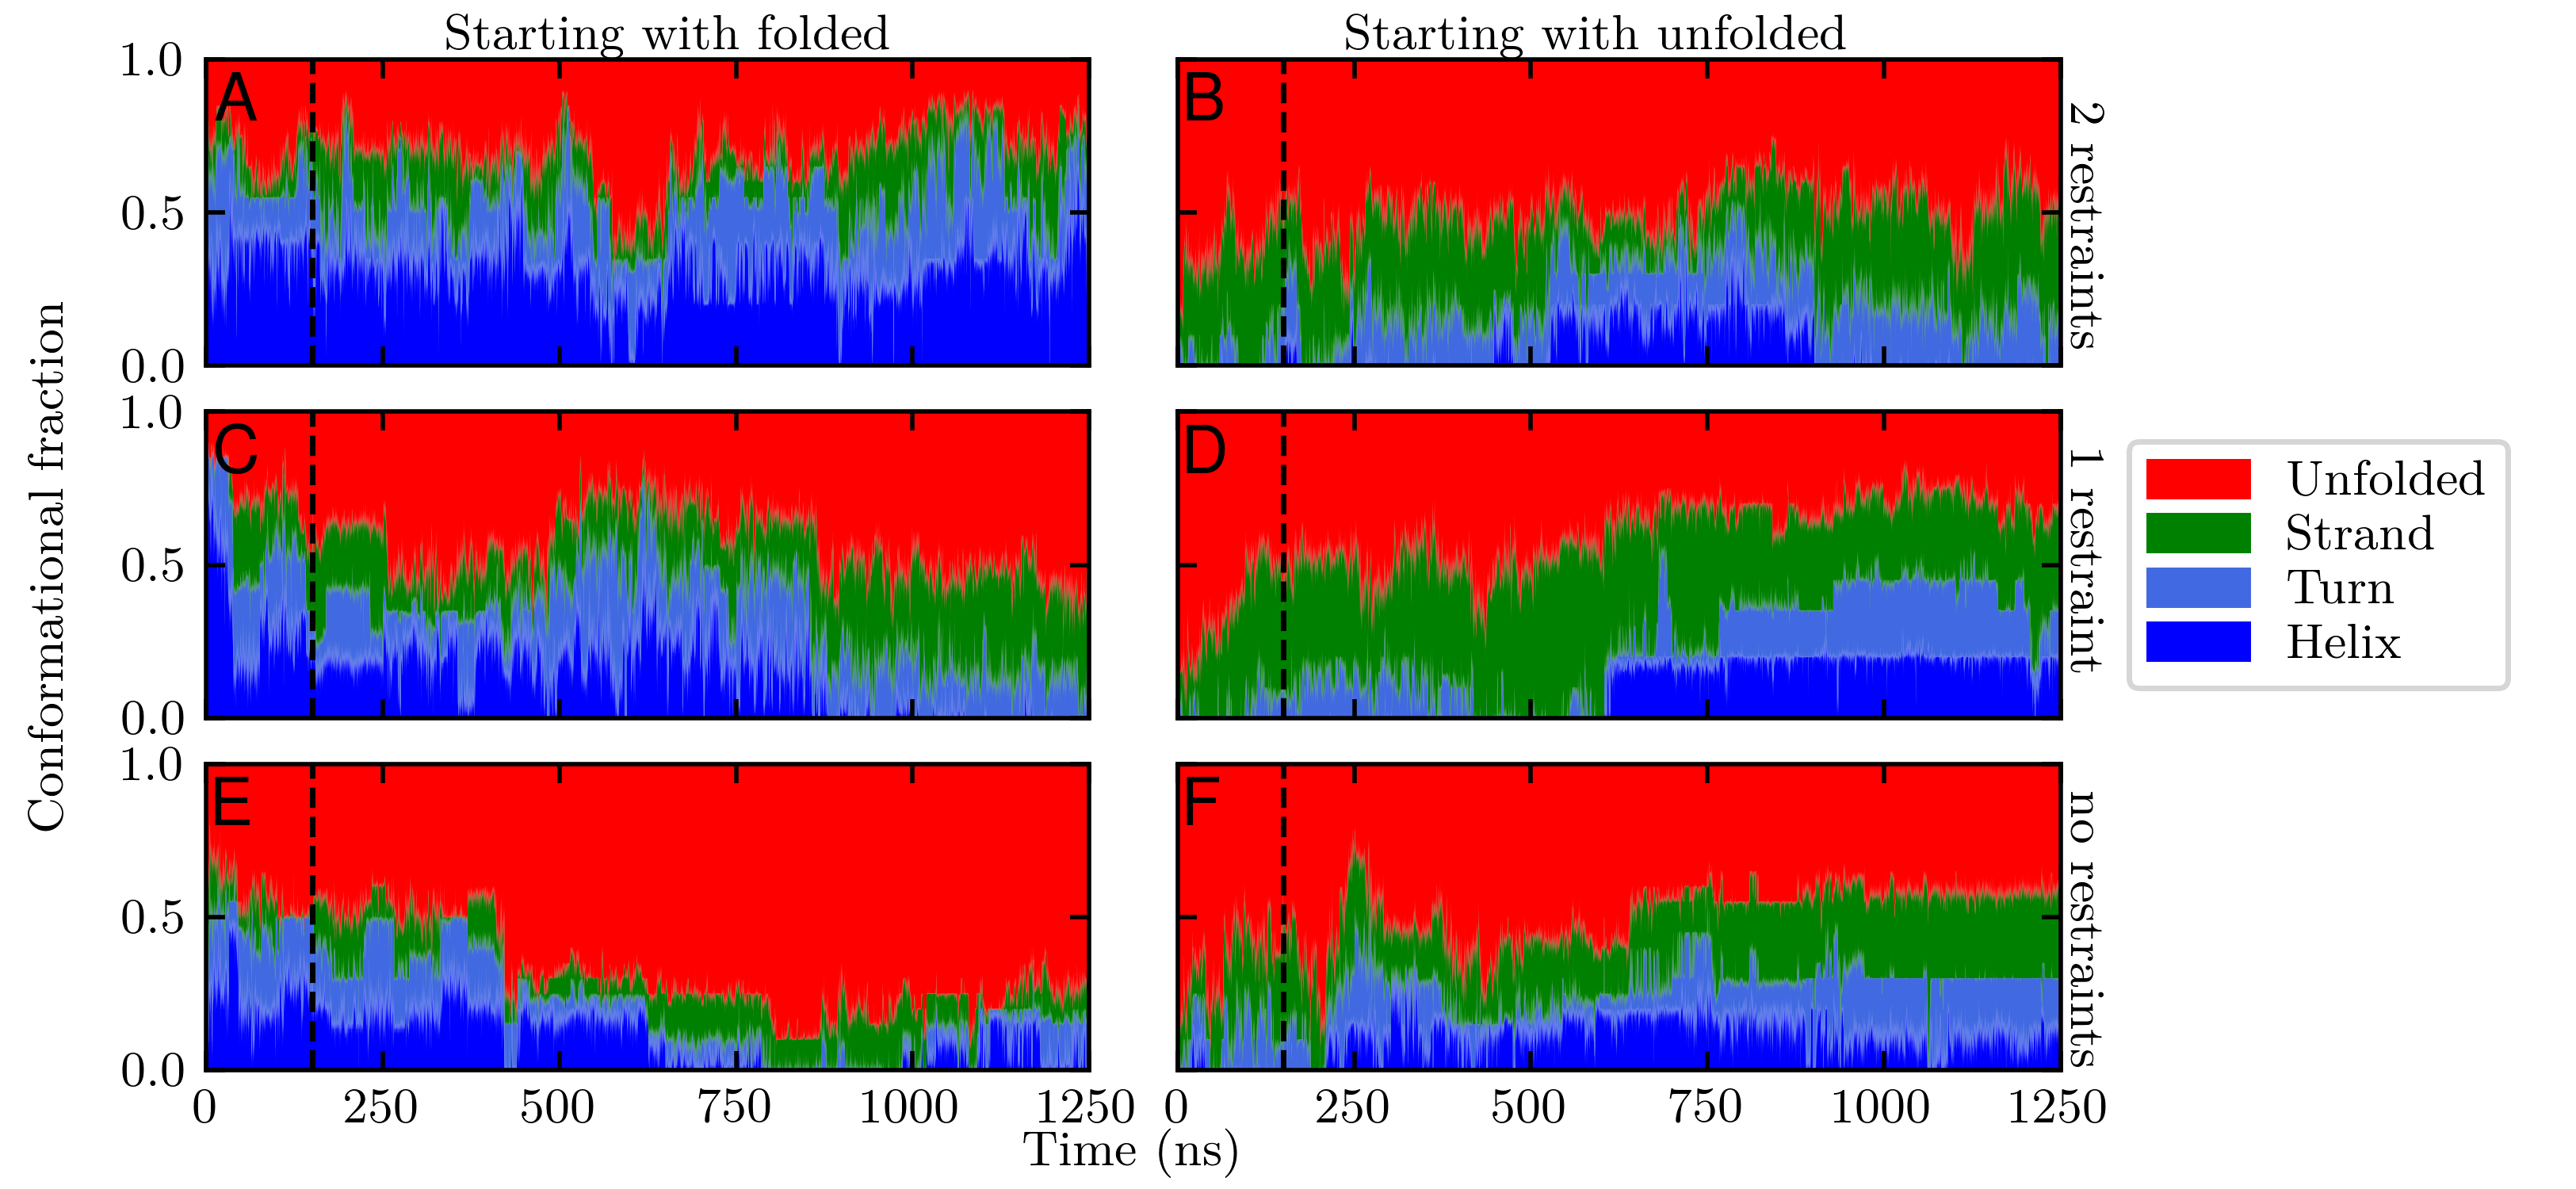
\includegraphics[width=\double]{figures-helix/disordered_helicity.png}
    \caption[Stacked conformational fractions of \pep{} on a disordered SAM]{
        Stacked conformational fractions of \pep{} on the surface of a \emph{disordered} SAM, with none, one, or two harmonic restraints between \pep{} and the SAM. 
        A, C, E: \pep{} began the simulation in an \textalpha{}-helical conformation. 
        B, D, F: \pep{} began the simulation unfolded. 
        A, B: \pep{} was harmonically restrained to the SAM at both glycine residues. 
        C, D: \pep{} was harmonically restrained to the SAM at only one of the glycine residues. 
        E, F: \pep{} was unrestrained on the SAM. 
        The black dashed lines represent the equilibration time. 
        The data after this mark was averaged and is presented in Table \ref{tbl:helix-disorder}. 
    }
    \label{fig:helix-disorder}
\end{figure}

\begin{table}
    \caption[Conformational fractions on the peptide on a disordered SAM]{Average conformational fractions from simulations of \pep{} on the surface of a \emph{disordered} SAM in which either none, one, or both of the glycine residues in the peptide are harmonically restrained to the SAM.}
    \begin{center}
     \resizebox{\double}{!}{
     \begin{tabular}{c|cccc|cccc}
     \toprule
         Number of  & \multicolumn{4}{c}{From folded} & \multicolumn{4}{c}{From unfolded} \\
         harmonic restraints & Helix & Turn & Strand & Unfolded & Helix & Turn & Strand & Unfolded \\
     \midrule
         2 & 0.322 & 0.218 & 0.159 & 0.302 & 0.052 & 0.156 & 0.291 & 0.501 \\
         1 & 0.140 & 0.188 & 0.230 & 0.442 & 0.110 & 0.134 & 0.368 & 0.388 \\
         0 & 0.103 & 0.091 & 0.116 & 0.689 & 0.125 & 0.145 & 0.239 & 0.490 \\
     \bottomrule
     \end{tabular}
    }
    \end{center}
    \label{tbl:helix-disorder}
\end{table}

For the case of the simulations that started from a folded conformation where the peptide was bound by a single restraint or not bound to the SAM, the peptide rapidly unfolded on the disordered SAM (Figures \ref{fig:helix-disorder}C,E). 
In both cases, leucine residues were observed to move to divots in the disordered SAM surface (see Figure \ref{fig:helix-disordered_sam}B), presumably to maximize hydrophobic interactions with the decanethiol molecules. 
This movement often broke hydrogen bonds in the peptide backbone, destabilizing the helix. 
When these simulations were started from an unfolded configuration, the peptide did not fold over the course of the simulation (Figures \ref{fig:helix-disorder}D,F). 
None of the simulations on the disordered SAM had average conformational fractions consistent with the simulations of \pep{} on an ordered SAM, with exception of the simulation that started with a folded conformation and both glycine residues bound. 
All had significantly lower helix (0.140 or less) and turn character (0.188 or less), and higher unfolded character (0.388 or greater) than the simulations on the ordered SAM. 
In order to investigate the underlying reasons for these conformational differences, we calculated the free energy surfaces of \pep{} on the ordered SAM and \pep{} on the disordered SAM from the combined ensembles of structures. 
The ensemble of structures for each of these surfaces were constructed using all frames from the simulations with either one restraint or no restraints. 
The simulations with two restraints were excluded because of the convergence issues discussed above. 
The free energy surface of \pep{} on the ordered SAM is shown in Figure \ref{fig:helix-free_order}A. 
There is a distinct minimum free energy of -23.1 kJ mol$^{-1}$ with low $R_g$ and low backbone RMSD to the \textalpha{}-helical conformation. 
By contrast, the free energy surface on the disordered SAM (shown in Figure \ref{fig:helix-free_order}B) contains a weaker minimum ($\Delta G = -20.1$ kJ mol$^{-1}$) with slightly higher RMSD and higher $R_g$, indicative of destabilization of the compact, helical conformation on the SAM. 
Importantly, while the free energy minimum of \pep{} on the ordered SAM was distinct, the free energy profile of \pep{} on the disordered SAM was more diffuse and the minima less apparent. 
From these results, we hypothesize that the molecular-level order of the SAM surface is a driving force in the folding of the peptide. 
Our hypothesis is consistent with recent work by Dallin et al. that demonstrated that the apparent hydrophobicity of a SAM surface decreases with more disorder \cite{Dallin2019}.   
Since \pep{} was designed to fold at a polar/apolar interface\cite{DeGrado1985} and hydrophobic surfaces can stabilize helices\cite{Levine2016}, a decrease in hydrophobicity of the SAM surface likely decreases the entropic gain of the hydrophobic interactions of the leucine residues with the SAM surface. 
The peptide must therefore distort from a stable helical secondary structure to achieve strong hydrophobic interactions between the leucines and the SAM decanethiol. 
This thereby increases the free energy of the folding process, resulting in the larger $\Delta G$ of the folded conformation observed in Figure \ref{fig:helix-free_order}B. 
Similar results have been reported for a shorter version of this peptide by Sprenger and Pfaendtner\cite{Sprenger2016}. 
We are currently investigating the dependence of the helical character of \pep{} on the extent of disorder of the SAM surface with additional simulations and experiments.  

\begin{figure}
    \center
    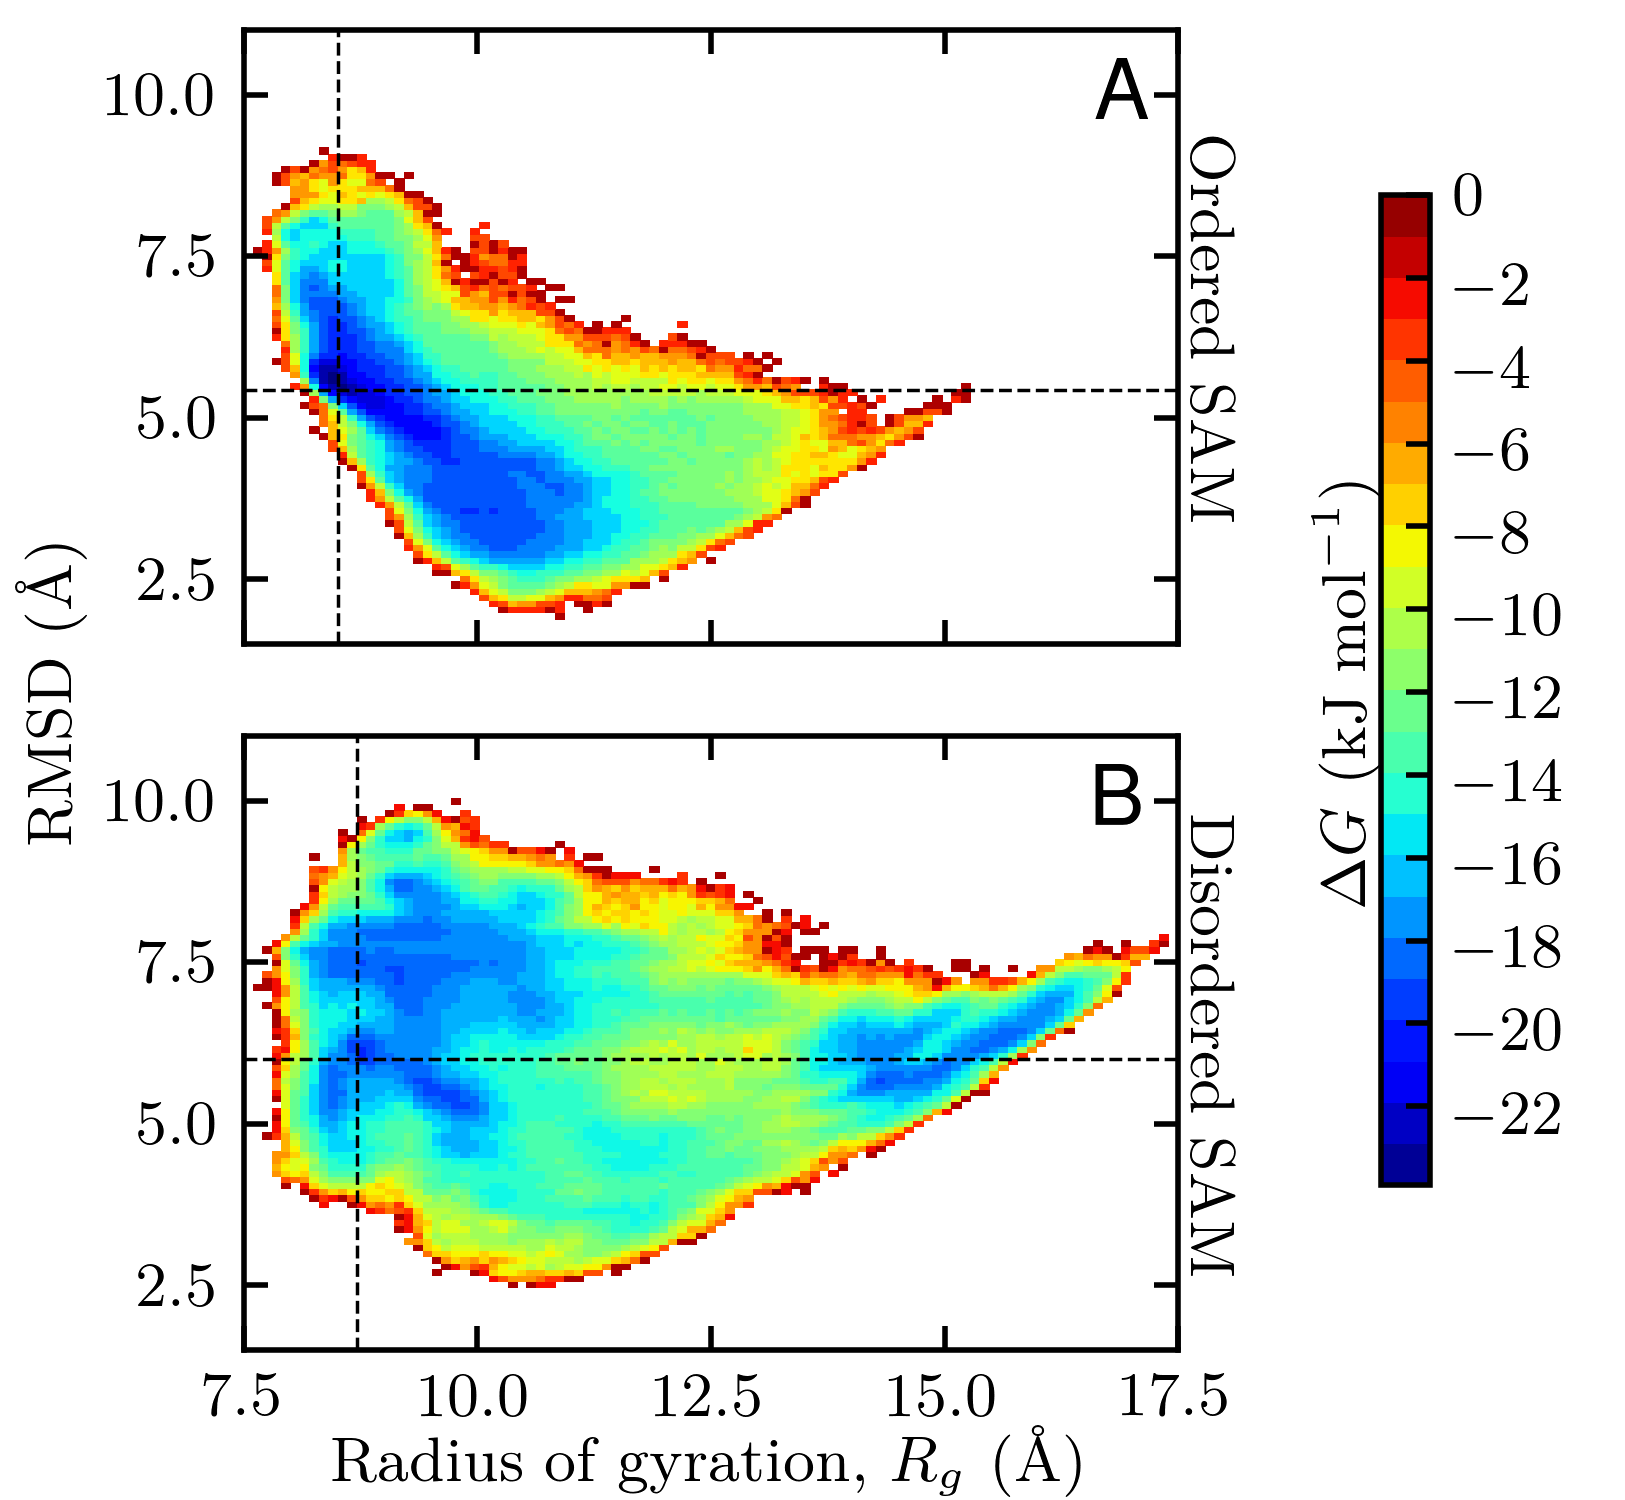
\includegraphics[width=\single]{figures-helix/comparison_free_energy_plots.png}
    \caption[Comparison of the free energy surfaces of \pep{} on an ordered SAM and on a disordered SAM]{
        Free energy surfaces of the combined ensembles of structures of \pep{} on the ordered SAM (A) and of \pep{} on the disordered SAM (B). 
        The combined ensembles exclude the trajectories with two restraints and structures prior to the equilibration time, as discussed in the main text. 
        On the $x$-axis is the radius of gyration of the protein. 
        On the $y$-axis is the backbone RMSD away from a perfectly folded \textalpha{}-helix. 
        The intersection of the dashed lines is the global minimum for each surface. 
    }
    \label{fig:helix-free_order}
\end{figure}

%%%%%%%%%%%%%%%%%%%%%%%%%%%%%%%%%%%%%%%%%%%%%%%%%%%%%%%%%%%%%%%%
%%%%%%%%%%%%%%%%%%%%%%%%%%%%%%%%%%%%%%%%%%%%%%%%%%%%%%%%%%%%%%%%
\section{Conclusion}\index{helix-conclusion}
%%%%%%%%%%%%%%%%%%%%%%%%%%%%%%%%%%%%%%%%%%%%%%%%%%%%%%%%%%%%%%%%
%%%%%%%%%%%%%%%%%%%%%%%%%%%%%%%%%%%%%%%%%%%%%%%%%%%%%%%%%%%%%%%%

The accuracy and applicability of canonical force fields such as OPLS-AA to complex environments is not automatic since these force fields were parameterized against structural information in the PDB, which is vastly overrepresented by compact globular proteins in dilute solution. 
However, using a set of 6 simulations of 1.25 \textmu{}s each of the charged peptide \pep{}, we demonstrated that widely available resources and the OPLS-AA force field were sufficiently accurate to describe the conformational change of our peptide induced by a binary solvent (\tbawat{}) and a SAM surface. 
We have demonstrated that while our simulations overestimated the amount of \textbeta{}-sheet character of the peptide in water, the conformational fractions from the simulations were quantitatively accurate to secondary structure estimates obtained from deconvoluting the experimental CD spectra. 
We further computed the CD spectra from the MD simulations, showing qualitative agreement with the experimental spectra. 
After demonstrating the accuracy of the simulations, we presented 10 additional 1.25 \textmu{}s simulations of \pep{} on the SAM surface under a variety of conditions. 
While we are unable to verify these final simulations with existing experimental data, they suggest two specific hypotheses about factors that may be important in peptide structure at a surface: 
1) the peptide must fold before the second covalent attachment to the surface; and 
2) the order of the SAM surface is a significant driving force to the folding process. 
These two hypotheses are currently being tested in our laboratory. 
While these results should not be extended arbitrarily to other systems, the ability to simulate accurate structural changes of biomolecules near surfaces or in otherwise complex environments has far reaching implications on plaque diseases, such as Alzheimer's disease, and can greatly aid in the incorporation of biomolecules onto surfaces for use in biosensors and catalytic devices. 



